% arara: indent: {overwrite: yes, silent: yes}
\documentclass[10pt]{amsart}
\input ../pree.tex

\begin{document}

\title{Recursive functions and models of computation}
\date{}
\maketitle

\section{Introduction}
\noindent
The goal of these notes is to formalize what constitutes an effective procedure. For this we introduce several models for computation. We consider models of two kinds: abstract and mechanical. Abstract models consist of partial recursive functions and functions defined by existential rudimentary formulas of the first-order language of arithmetic. Among the mechanical models we have Loop-while programs, register machines and Turing-Post machines. We prove that they are all equivalent in expressive power. Moreover, all notions introduced in these notes are formulated from the beginning in a way that naturally relativizes to oracles.

\section{Partial functions and relations on powers of natural numbers}
\noindent
This section introduces terminology used throughout the notes.

The set of all natural numbers is $\NN$. Note that $\NN$ is well ordered by the standard relation $\leq$. By an initial interval of $\NN$ we mean an initial segment with respect to $\leq$.

If $k \in \NN$, then the set of $k$-tuples of numbers is the Cartesian product $\NN^k$. We denote $k$-tuples of numbers by vector notation $\vec{n}$ and refer to the number $k$ as the length of $\vec{n}$. In the case $k = 0$ the set $\NN^0$ contains a unique element: the empty tuple.

\begin{definition}
	Let $k\in \NN$. Let $f$ be a function with domain a subset of $\NN^k$ and taking values in $\NN$. Then $f$ is a \textit{$k$-ary partial function}.
\end{definition}

\begin{definition}
	A \textit{partial function} is a $k$-ary partial function for some $k \in \NN$.
\end{definition}

\begin{definition}
	Let $f$ be a $k$-ary partial function. If $\vec{n} \in \NN^k$ is in the domain of $f$, then we say that $f$ is \textit{defined at $\vec{n}$}.
\end{definition}

\begin{remark}\label{remark:up_and_down_arrows_for_arguments_of_definition}
	Let $f$ be a $k$-ary partial function and let $\vec{n} \in \NN^k$. We write $f(\vec{n})\downarrow$ to denote that $f$ is defined at $\vec{n}$. If $f$ is not defined at $\vec{n}$, then we use $f(\vec{n})\uparrow$.
\end{remark}

\begin{definition}
	Let $k \in \NN$ and let $f$ be a $k$-ary partial function. Then
	$$\Gamma_f = \big\{\left(\vec{n},f(\vec{n})\right)\in \NN^{k+1}\,\big|\mbox{ for }\vec{n} \in \NN^k\mbox{ such that }f(\vec{n})\downarrow\big\}$$
	is \textit{the graph} of $f$.
\end{definition}

\begin{definition}
	Let $f$ be a $k$-ary partial function such that $f(\vec{n})\downarrow$ for every $\vec{n} \in \NN^k$. Then $f$ is called a \textit{$k$-ary total function}.
\end{definition}

\begin{definition}
	Let $g$ be a $k$-ary partial function and let $f_1,...,f_k$ be $l$-ary partial functions. Consider all $\vec{n} \in \NN^l$ such that $f_1(\vec{n})\downarrow,...,f_k(\vec{n})\downarrow$ and $g\big(f_1(\vec{n}),...,f_k(\vec{n})\big)\downarrow$. Then the map
	$$\vec{n} \mapsto g\big(f_1(\vec{n}),...,f_k(\vec{n})\big)$$
	gives rise to a well defined $l$-ary partial function. We refer to this partial function as the \textit{composition of $g$ with $f_1,...,f_k$}.
\end{definition}

\begin{definition}
	Let $g$ be a $(k + 2)$-ary partial function and let $f$ be a $k$-ary partial function for some $k \in \NN$. Fix $\vec{n} \in \NN^k$. We define $h(\vec{n},m)$ for numbers $m$ in some initial interval of $\NN$. We set
	$$h(\vec{n},0) = f(\vec{n})$$
	if $f(\vec{n})\downarrow$. Now suppose that $h(\vec{n},m)\downarrow$ for some number $m$ and that $g\big(\vec{n}, m, h\left(\vec{n},m\right)\big)\downarrow$. Then we set
	$$h(\vec{n}, m + 1) = g\big(\vec{n}, m, h\left(\vec{n},m\right)\big)$$
	Then $h$ is a $(k+1)$-ary partial function obtained by \textit{primitive recursion} from $g$ and $f$.
\end{definition}

\begin{definition}
	Let $g$ be a $(k + 1)$-ary partial function for some $k \in \NN$. Fix $\vec{n} \in \NN^k$. Suppose that there exists number $l$ such that
	$$g\left(\vec{n},0\right)\downarrow,g\left(\vec{n},1\right)\downarrow,...,g\left(\vec{n},l - 1\right)\downarrow$$
	are defined, nonzero numbers and $g(\vec{n},l) = 0$. Then we define $\mu_m \big[g\left(\vec{n},m\right) = 0\big] = l$. If such number $l$ does not exist, then $\mu_m \big[g\left(\vec{n},m\right) = 0\big]$ is undefined. This gives rise to a $k$-ary partial function $\mu_m \big[g(\vec{n}, m) = 0\big]$ called the \textit{unbounded minimization} of $g$.
\end{definition}
\noindent
We also need some terminology concerning relations.

\begin{definition}
	Let $k\in \NN$ and let $R\subseteq \NN^k$. Then $R$ is a \textit{$k$-ary relation}.
\end{definition}

\begin{definition}
	Let $k \in \NN$ and let $R$ be a $k$-ary relation. The $k$-ary function
	$$
		\mathbb{1}_R\left(\vec{n}\right) = \begin{cases}
			1 & \mbox{ if }\vec{n} \in R \\
			0 & \mbox{ otherwise }       \\
		\end{cases}
	$$
	is called the \textit{characteristic function} of $R$.
\end{definition}

\begin{definition}
	Let $R$ be a $k$-ary relation. Let $c_R$ be partial function such that $c_R(\vec{n}) = 1$ for all $\vec{n} \in R$ and $c_R(\vec{n})\uparrow$ otherwise. Then $c_R$ is the \textit{semicharacteristic function} of $R$.
\end{definition}
\noindent
Next we introduce some notions concerning class of functions.

\begin{definition}
	Let $\cF$ be a class of partial functions.
	\begin{enumerate}[label=\textbf{(\arabic*)}, leftmargin=3.0em]
		\item Suppose that for every positive $k \in \NN$, every $k$-ary partial function $g \in \cF$ and all partial functions $f_1,...,f_k\in \cF$ of the same arity the composition of $g$ with $f_1,...,f_k$ is in $\cF$. Then $\cF$ is \textit{closed under composition}.
		\item Suppose that for every positive $k \in \NN$, every $(k+2)$-ary partial function $g\in \cF$ and every $k$-ary partial function $f\in \cF$ the function obtained by primitive recursion from $g$ and $f$ is in $\cF$. Then $\cF$ is \textit{closed under primitive recursion}.
		\item Suppose that for every positive $k \in \NN$ and every $(k+1)$-ary partial function $g\in \cF$ the function $\mu_m\big[g(\vec{n},m) = 0\big]$ is in $\cF$. Then $\cF$ is \textit{closed under unbounded minimization}.
	\end{enumerate}
\end{definition}
\noindent
Finally, we use the following notation. For every $k \in \NN$ we denote by $Z_k$ the function given by formula $\vec{n} \mapsto 0$ for each $\vec{n} \in \NN^k$. We denote by $s$ the successor function i.e. $s(n) = n + 1$ for $n \in \NN$. For every positive $k \in \NN$ and each $i \in \NN$ such that $1\leq i \leq k$ we denote by $I^i_k$ the projection $\vec{n} \mapsto n_i$ where $\vec{n} = \left(n_1,...,n_k\right) \in \NN^k$.

\section{Primitive recursive functions}

\begin{definition}
	The class of \textit{primitive recursive functions} is the smallest class of partial functions that contains:
	\begin{enumerate}[label=\textbf{(\arabic*)}, leftmargin=3.0em]
		\item the successor $s$,
		\item $Z_k$ for every $k \in \NN$,
		\item $I^i_k$ for every positive $k \in \NN$ and $1\leq i \leq k$,
	\end{enumerate}
	and is closed under composition and primitive recursion.
\end{definition}

\begin{proposition}\label{proposition:all_primitive_recursive_functions_are_total}
	All primitive recursive functions are total.
\end{proposition}
\begin{proof}
	Note that the class of total functions is closed under composition and primitive recursion. Since the class of primitive recursive functions  is defined by these operations, it follows that all primitive recursive functions  are total.
\end{proof}
\noindent
The remainder of this section is devoted to proving that most well-known total functions are primitive recursive.

\begin{proposition}\label{proposition:all_constant_functions_are_primitive_recursive}
	Then all $k$-ary total constant functions are primitive recursive  for every $k \in \NN$.
\end{proposition}
\begin{proof}
	Let $j$ be a number. By composing the successor function with itself $j$-times we obtain the function $n \mapsto n + j$, which is primitive recursive. Next by composing this function with the zero $k$-ary function, we derive the $k$-ary total constant function with $j$ as the only value. Hence this function is also primitive recursive. This completes the proof.
\end{proof}

\begin{proposition}\label{proposition:addition_is_primitive_recursive}
	The addition function $(n,m) \mapsto n + m$ is primitive recursive.
\end{proposition}
\begin{proof}
	The identity function is primitive recursive. Similarly the function $(n,m,l) \mapsto l + 1$ is primitive recursive. Next the function $(n,m) \mapsto n + m$ is obtained by primitive recursion from the two functions described above.
\end{proof}

\begin{proposition}\label{proposition:multiplication_is_primitive_recursive}
	The multiplication function $(n,m) \mapsto n\cdot m$ is primitive recursive.
\end{proposition}
\begin{proof}
	Note that the function $(n,m,l)\mapsto n + l$ is the composition of addition function with projections on first and last factor. Hence it is primitive recursive. Next observe that the function $(n,m)\mapsto n\cdot m$ is obtained by primitive recursion from $(n,m,l) \mapsto n + l$ and the zero unary function.
\end{proof}

\begin{proposition}\label{proposition:power_function_is_primitive_recursive}
	The exponential function $(n,m) \mapsto n^m$ is primitive recursive.
\end{proposition}
\begin{proof}
	Note that the function $(n,m,l) \mapsto n\cdot l$ is the composition of multiplication with projections on first and last factors. Hence it is primitive recursive  by Proposition \ref{proposition:multiplication_is_primitive_recursive}. Now the function $(n, m) \mapsto n^m$ is obtained by primitive recursion from $(n,m,l) \mapsto n\cdot l$ and constant unary function with value $1$. Since both these functions are primitive recursive, the proof is completed.
\end{proof}

\begin{definition}
	The function
	$$n \mapsto \begin{cases}
			n - 1 & \mbox{ if }n > 0   \\
			0     & \mbox{ otherwise } \\
		\end{cases}$$
	is the \textit{predecessor} function.
\end{definition}

\begin{proposition}\label{proposition:predecessor_function_is_primitive_recursive}
	The predecessor function is primitive recursive.
\end{proposition}
\begin{proof}
	The predecessor function is obtained by primitive recursion from the $2$-ary projection on the first factor and the zero nullary function. Hence it is primitive recursive.
\end{proof}

\begin{definition}
	The $2$-ary function
	$$n \dotminus m = \begin{cases}
			n - m & \mbox{ if }n > m   \\
			0     & \mbox{ otherwise }
		\end{cases}$$
	is the \textit{monus} function.
\end{definition}

\begin{proposition}\label{proposition:monus_function_is_primitive_recursive}
	The monus function is primitive recursive.
\end{proposition}
\begin{proof}
	Note that the function $(n,m,l) \mapsto l\dotminus 1$ is the composition of the predecessor with the projection on the last factor. By Proposition \ref{proposition:predecessor_function_is_primitive_recursive} it is primitive recursive. The monus function is obtained from $(n,m,l)\mapsto l \dotminus 1$ and the identity by primitive recursion. Thus it is primitive recursive.
\end{proof}

\begin{proposition}\label{proposition:fold_mechanism_for_sum_and_product_is_primitive_recursive}
	Let $k\in \NN$ and let $f$ be a $(k+1)$-ary primitive recursive function. Then functions
	$$(\vec{n},m)\mapsto \sum_{l < m}f(\vec{n},l),\,(\vec{n},m) \mapsto \prod_{l < m}f(\vec{n},l)$$
	are primitive recursive.
\end{proposition}
\begin{proof}
	We prove the result for sum. The proof for product is analogous.

	First observe that the function $(\vec{n},m,l) \mapsto f(\vec{n},m)$ is the composition of $f$ and $I^{k+2}_1,...,I^{k+2}_{k+1}$. Hence it is primitive recursive. Next note that the function $(\vec{n},m,l) \mapsto l + f(\vec{n},m)$ is primitive recursive  as the composition of addition with the function described above and $I^{k+2}_{k+2}$. Finally the function
	$$(\vec{n},m)\mapsto \sum_{l < m}f(\vec{n},l)$$
	is obtained by primitive recursion from the function described above and the $k$-ary zero function.
\end{proof}

\begin{corollary}\label{corollary:fold_mechanism_for_sum_and_product_is_primitive_recursive}
	Let $k\in \NN$ and let $f$ be a $(k + 1)$-ary primitive recursive function. Then functions given by formulas
	$$(\vec{n},m)\mapsto \sum_{l \leq m}f(\vec{n},l),\,(\vec{n},m) \mapsto \prod_{l \leq m}f(\vec{n},l)$$
	are primitive recursive.
\end{corollary}
\begin{proof}
	Left for the reader as an exercise.
\end{proof}

\begin{definition}
	The function
	$$\mathrm{sign}(n) = \begin{cases}
			1 & \mbox{ if }n > 0   \\
			0 & \mbox{ otherwise } \\
		\end{cases}$$
	is the \textit{sign} function.
\end{definition}

\begin{proposition}\label{proposition:zery_indicator_is_primitive_recursive}
	The sign function is primitive recursive.
\end{proposition}
\begin{proof}
	The sign function is obtained by primitive recursion from the constant $2$-ary function with value $1$ and the nullary zero function. Since both these functions are primitive recursive, we obtain the statement.
\end{proof}

\section{Primitive recursive relations}

\begin{definition}
	Let $R$ be a $k$-ary relation for some $k \in \NN$. Suppose that the characteristic function of $R$ is primitive recursive. Then $R$ is \textit{primitive recursive}.
\end{definition}

\begin{proposition}\label{proposition:primitive_recursive_relations_form_boolean_algebra}
	Let $k\in \NN$ and let $R, S$ be $k$-ary primitive recursive relations. Then the following assertions hold.
	\begin{enumerate}[label=\emph{\textbf{(\arabic*)}}, leftmargin=*]
		\item $R \cup S$ is primitive recursive.
		\item $R \cap S$ is primitive recursive.
		\item $\NN^k \setminus R$ is primitive recursive.
	\end{enumerate}
\end{proposition}
\begin{proof}
	For the proof of \textbf{(1)} note that the function obtained by applying sign to the sum $\mathbb{1}_R + \mathbb{1}_{S}$ is primitive recursive. Since this function coincides with $\mathbb{1}_{R\cup S}$, we derive that \textbf{(1)} holds.

	Since $\mathbb{1}_{R\cap S} = \mathbb{1}_{R}\cdot \mathbb{1}_S$, we deduce that \textbf{(2)} holds.

	Let $\mathbb{1}_{\NN^k}$ be a constant $k$-ary function with value $1$. By composing monus function with $\mathbb{1}_{\NN^k}, \mathbb{1}_R$ we deduce that $$\mathbb{1}_{\NN^k\setminus R} = \mathbb{1}_{\NN^k} \dotminus \mathbb{1}_R$$
	is primitive recursive. This proves \textbf{(3)}.
\end{proof}

\begin{proposition}\label{proposition:bounded_quantifiers_are_primitive_recursive}
	Let $k\in \NN$ and let $R$ be a $(k + 1)$-ary primitive recursive relation. Then
	$$\big\{(\vec{n},m) \in \NN^{k+1}\,\big|\,(\vec{n},l)\in R\mbox{ for all }l < m\big\},\,\big\{(\vec{n},m) \in \NN^{k+1}\,\big|\,(\vec{n},l)\in R\mbox{ for all }l \leq m\big\},$$
	$$\big\{(\vec{n},m) \in \NN^{k+1}\,\big|\,(\vec{n},l)\in R\mbox{ for some }l < m\big\},\,\big\{(\vec{n},m) \in \NN^{k+1}\,\big|\,(\vec{n},l)\in R\mbox{ for some }l < m\big\}$$
	are primitive recursive.
\end{proposition}
\begin{proof}
	This follows immediately from Proposition \ref{proposition:fold_mechanism_for_sum_and_product_is_primitive_recursive} and Corollary \ref{corollary:fold_mechanism_for_sum_and_product_is_primitive_recursive} combined with the fact that sign is primitive recursive.
\end{proof}

\begin{proposition}\label{proposition:order_relations_are_primitive_recursive}
	The binary relations $<,\leq,=$ are primitive recursive.
\end{proposition}
\begin{proof}
	The relation $<$ is primitive recursive  because its characteristic function can be expressed by combination of monus and sign which are primitive recursive functions. By Proposition \ref{proposition:primitive_recursive_relations_form_boolean_algebra} the relation $\geq$  is primitive recursive  as well. Since
	$$\big\{(n,m) \in \NN^2\,\big|\,n \leq m\big\}$$
	is obtained  by swapping variables in
	$$\big\{(m,n) \in \NN^2\,\big|\,n\geq m \big\}$$
	it is also primitive recursive. Finally using Proposition \ref{proposition:primitive_recursive_relations_form_boolean_algebra} and the fact that intersection of relation above is the diagonal of $\NN^2$ we derive the statement.
\end{proof}
\noindent
Now we prove some useful results regarding primitive recursive relations and functions.

\begin{proposition}\label{proposition:primitive_recursive_alternative_produces_primitive_recursive_function}
	Let $k, m \in \NN$. Let $R_1,...,R_m$ be $k$-ary primitive recursive relations  and let $f_1,...,f_m$ be $k$-ary primitive recursive functions. Suppose that
	$$\NN^k = R_1\cup... \cup R_m$$
	is a decomposition onto pairwise disjoint sets. Then the $k$-ary function defined by
	$$\vec{n} \mapsto
		\begin{cases}
			f_1(\vec{n}) & \mbox{ if }\vec{n} \in R_1 \\
			...                                       \\
			f_m(\vec{n}) & \mbox{ if }\vec{n} \in R_m \\
		\end{cases}$$
	is primitive recursive.
\end{proposition}
\begin{proof}
	Indeed, we have
	$$f(\vec{n}) = f_1(\vec{n})\cdot \mathbb{1}_{R_1}(\vec{n}) +... + f_m(\vec{n})\cdot \mathbb{1}_{R_m}(\vec{n})$$
	for every $\vec{n} \in \NN^k$.
\end{proof}

\begin{definition}
	Let $k \in \NN$ and let $R$ be a $(k + 1)$-ary relation. We define
	$$\mu_{l < m}\big[(\vec{n},l) \in R\big] =
		\begin{cases}
			\min \{l\,|\,l < m\mbox{ and }(\vec{n},l)\in R\} & \mbox{ if }(\vec{n},l)\in R\mbox{ for some }l < m \\
			m                                                & \mbox{ otherwise }                                \\
		\end{cases}
	$$
	Then $\mu_{l < m}\big[(\vec{n},l) \in R\big]$ is said to be obtained by \textit{bounded minimization} from $R$.
\end{definition}
\noindent
Finally we prove important result that bounded minimization of primitive recursive relation  is primitive recursive function.

\begin{proposition}\label{proposition:bounded_minimization_is_primitive_recursive_if_relation_is_primitive_recursive}
	Let $k \in \NN$ and let $R$ be a $(k + 1)$-ary primitive recursive relation. Then the function
	$$(\vec{n},m)\mapsto \mu_{l < m}\big[(\vec{n},l) \in R\big]$$
	is primitive recursive.
\end{proposition}
\begin{proof}
	Define a relation
	$$N = \big\{(\vec{n},m)\in \NN^k\,\big|\,(\vec{n},l) \not \in R\mbox{ for all }l < m\big\}$$
	Then $N$ is the $(k+1)$-ary primitive recursive relation  by Proposition \ref{proposition:bounded_quantifiers_are_primitive_recursive}. Next $S = N\cap R$ is a primitive recursive $(k+1)$-ary relation  such that $(\vec{n},m) \in S$ if and only if $m$ is the smallest number such that $(\vec{n},m) \in R$. Now observe that
	$$\mu_{l < m}\big[(\vec{n},l)\in R\big] = m\cdot \mathbb{1}_N\left(\vec{n},m\right) + \sum_{l < m}l \cdot \mathbb{1}_{S}\left(\vec{n},l\right)$$
	for every $\vec{n} \in \NN^k$ and $m \in \NN$. This function is primitive recursive  by Proposition \ref{proposition:fold_mechanism_for_sum_and_product_is_primitive_recursive}, the fact that sum is primitive recursive  and our observations that $N,S$ are primitive recursive $(k + 1)$-ary relations.
\end{proof}

\section{Number theory and primitive recursion}
\noindent
In this section we focus on some elementary number-theoretic properties and their relation to primitive recursion.

\begin{proposition}\label{proposition:divisibility_is_primitive_recursive}
	The divisibility relation $\mid$ is primitive recursive.
\end{proposition}
\begin{proof}
	We have $n\mid m$ if and only if $l\cdot n = m$ for some $l \leq m$. Hence divisibility is primitive recursive by Proposition \ref{proposition:bounded_quantifiers_are_primitive_recursive}.
\end{proof}

\begin{proposition}\label{proposition:prime_numbers_are_primitive_recursive}
	The set $\mathbb{P}$ of prime numbers is primitive recursive.
\end{proposition}
\begin{proof}
	We have
	$$\mathbb{P} = \big\{p \in \NN\,\big|\,p > 1\mbox{ and }p\mbox{ is not divisible by }n\mbox{ for all }1 < n < p\big\}$$
	Hence $\mathbb{P}$ is primitive recursive by results of previous section.
\end{proof}

\begin{theorem}\label{theorem:prime_sequence_is_primitive_recursive}
	Let $p_n$ denote the $n$-th prime number. Then the function $n \mapsto p_n$ is primitive recursive.
\end{theorem}
\noindent
For the proof we need some elementary result.

\begin{lemma}\label{lemma:factorial_is_primitive_recursive}
	The factorial function $n \mapsto n!$ is primitive recursive.
\end{lemma}
\begin{proof}[Proof of the lemma]
	Left for the reader as an exercise.
\end{proof}

\begin{proof}[Proof of the theorem]
	Consider the total $2$-ary function
	$$f(n, m) = \mu_{l < m}\,\big[\left(n < l\right)\mbox{ and }l \in \mathbb{P}\big]$$
	According to Proposition \ref{proposition:prime_numbers_are_primitive_recursive} and Proposition \ref{proposition:bounded_minimization_is_primitive_recursive_if_relation_is_primitive_recursive} we infer that $f$ is primitive recursive. By Lemma \ref{lemma:factorial_is_primitive_recursive} we derive that
	$$g(n) = f(n,n!+2)$$
	is primitive recursive. Note that $g(n)$ is the smallest prime number greater than $n$.

	Now we have $p_0 = 2$ and
	$$p_{n+1} = g(p_n)$$
	for every $n$. Hence $n \mapsto p_n$ is obtained by primitive recursion from $g\cdot I^2_2$ and constant function equal to $2$. Therefore, it is primitive recursive.
\end{proof}

\begin{proposition}\label{proposition:prime_exponent_is_primitive_recursive}
	For numbers $n,m$ we define
	$$e_{m}(n) = \begin{cases}
			\max \big\{l\,|\,p_m^l\mbox{ divides }n\big\} & \mbox{ if }n > 0 \\
			0                                             & \mbox{ if }n = 0 \\
		\end{cases}
	$$
	Then the function $(n,m) \mapsto e_{m}(n)$ is primitive recursive.
\end{proposition}
\begin{proof}
	Suppose that $n > 0$. Then
	$$e_m(n) = \mu_{l < n}\left[n\mbox{ is not divisible by }p_m^l\right] \dotminus 1$$
	for all $m \in \NN$. Clearly $e_m(0) = 0$ for all $m \in \NN$. Hence results of the previous section and the fact that the monus is primitive recursive imply that $(n,m) \mapsto e_{m}(n)$ is primitive recursive.
\end{proof}

\section{Primitive recursive encoding of sequences}
\noindent
In this section we explore how finite sequences of natural numbers can be represented and manipulated within the framework of primitive recursive functions. We will define encoding schemes for sequences and demonstrate that common operations on sequences are primitive recursive.

\begin{definition}
	We define
	$$\pmb{[}\vec{n}\pmb{]} = \begin{cases}
			p_0^{1 + n_0}\cdot...\cdot p_{k}^{1 + n_k} & \mbox{ if }\vec{n} = \left(n_0,...,n_k\right)\in \NN^{k + 1}\mbox{ for some }k \\
			1                                          & \mbox{ if }\vec{n}\mbox{ is empty tuple}                                       \\
		\end{cases}
	$$
	Then $\pmb{[}\vec{n}\pmb{]}$ is the \textit{sequence number of $\vec{n}$}.
\end{definition}

\begin{proposition}\label{proposition:tuple_codes_are_primitive_recursive}
	Let $\mathrm{Seq}$ denote the set of sequence numbers of all tuples. Then $\mathrm{Seq}$ is a primitive recursive set.
\end{proposition}
\begin{proof}
	We have
	$$\mathrm{Seq} = \big\{n \in \NN\big|\,n > 0\mbox{ and for all }l < n\mbox{ either }e_l(n) = 0\mbox{ or }e_l(n) \geq 1\bigg)$$
	Hence $\mathrm{Seq}$ is primitive recursive.
\end{proof}

\begin{definition}
	We define
	$$\mathrm{lh}(n) = \begin{cases}
			k & \mbox{ if }n = \pmb{[}\vec{n}\pmb{]}\mbox{ for some }\vec{n} \in \NN^k \\
			0 & \mbox{ otherwise }                                                     \\
		\end{cases}
	$$
	Then $\mathrm{lh}(n)$ is the \textit{length} of $n$.
\end{definition}

\begin{proposition}\label{proposition:length_is_primitive_recursive}
	The function $n \mapsto \mathrm{lh}(n)$ is primitive recursive.
\end{proposition}
\begin{proof}
	Consider set
	$$\mathbb{P}_n = \big\{l \in \NN\,\big|\,p_l|n\big\}$$
	of indexes of prime divisors of $n$. Then function
	$$n \mapsto \sum_{l < n}\mathbb{1}_{\mathbb{P}_n}(l)$$
	is primitive recursive. Note that
	$$\mathrm{lh}(n) = \begin{cases}
			\sum_{l < n}\mathbb{1}_{\mathbb{P}_n}(l) & \mbox{ if }n \in \mathrm{Seq} \\
			0                                        & \mbox{ otherwise }
		\end{cases}$$
	Hence $\mathrm{lh}$ is primitive recursive and the proposition is proved.
\end{proof}

\begin{proposition}\label{proposition:sequence_element_access_is_primitive_recursive}
	For numbers $n, l \in \NN$ define
	$$n[l] = \begin{cases}
			n_l & \mbox{ if }n = \pmb{[}\vec{n}\pmb{]}\mbox{ for some }k\in \NN,\vec{n}\in \NN^{k + 1}\mbox{ and }0 \leq l \leq k \\
			0   & \mbox{ otherwise }                                                                                              \\
		\end{cases}$$
	Then the function $(n,l) \mapsto n[l]$ is primitive recursive.
\end{proposition}
\begin{proof}
	We have
	$$n[l] = \begin{cases}
			e_{l}(n) \dotminus 1 & \mbox{ if }n \in \mathrm{Seq}\mbox{ and }0\leq l < \mathrm{lh}(n) \\
			0                    & \mbox{ otherwise }                                                \\
		\end{cases}$$
	and hence the proposition follows.
\end{proof}

\begin{proposition}\label{proposition:sequence_encoding_is_primitive_recursive_function}
	Let $k\in \NN$. Then the $k$-ary function
	$$\NN^k\ni \vec{n} \mapsto \pmb{[}\vec{n}\pmb{]}\in \NN$$
	is primitive recursive.
\end{proposition}
\begin{proof}
	Left for the reader.
\end{proof}
\noindent
Suppose that $n,m\in \mathrm{Seq}$. Then $n\star m$ is a sequence number such that
$$\mathrm{lh}(n\star m) = \mathrm{lh}(n) + \mathrm{lh}(m)$$
and
$$\left(n\star m\right)[l] = \begin{cases}
		n[l]                  & \mbox{ if }0\leq l < \mathrm{lh}(n)                                \\
		m[l - \mathrm{lh}(n)] & \mbox{ if }\mathrm{lh}(n) \leq l < \mathrm{lh}(n) + \mathrm{lh}(m) \\
	\end{cases}$$
Moreover, if one of $n,m\in \NN$ is not a sequence number, then we set $n\star m = 0$.

\begin{proposition}\label{proposition:concatenation_is_primitive_recursive}
	The function $(n,m) \mapsto n\star m$ is primitive recursive.
\end{proposition}
\begin{proof}
	Suppose that $n,m \in \mathrm{Seq}$. Then
	$$n\star m = n \cdot \prod_{l < \mathrm{lh}(m)}p_{\mathrm{lh}(n) + l}^{1 + m[l]}$$
	and hence $(n,m) \mapsto n\star m$ is primitive recursive.
\end{proof}

\section{Recursive functions relative to subset}
\noindent
First we introduce the relative version of primitive recursive functions.

\begin{definition}
	Let $A$ be a subset of $\NN$. The class of \textit{primitive recursive functions relative to $A$} is the smallest class of partial recursive functions which contains:
	\begin{enumerate}[label=\textbf{(\arabic*)}, leftmargin=3.0em]
		\item the successor $s$,
		\item $Z_k$ for every $k \in \NN$,
		\item $I^i_k$ for every positive $k \in \NN$ and $1\leq i \leq k$,
		\item the characteristic function $\mathbb{1}_A$ of $A$,
	\end{enumerate}
	and is closed under composition and primitive recursion.
\end{definition}

\begin{definition}
	Let $R$ be a $k$-ary relation for some $k \in \NN$ and let $A$ be a subset of $\NN$. Suppose that the characteristic function of $R$ is primitive recursive relative to $A$. Then $R$ is \textit{primitive recursive relative to $A$}.
\end{definition}

\begin{remark}\label{remark:primitive_recursive_relative_to_subset_have_all_nice_properties}
	Let $A$ be a subset of $\NN$. Note that all results proved in previous sections for primitive recursive functions and relations hold for primitive recursive functions and relations relative to $A$.
\end{remark}

\begin{remark}\label{remark:primitive_recursive_are_primitive_recursive_relative_to_empty_set}
	Observe that primitive recursive functions coincide with the class of primitive recursive functions relative to $\emptyset$.
\end{remark}
\noindent
We introduce a class of functions, which naturally extends the class of primitive recursive functions. It was defined by Herbrand and G{\"o}del in the early 1930s after publication of \cite{godel1931formal}. After that it was further clarified by Kleene.

\begin{definition}
	Let $A$ be a subset of $\NN$. The class of \textit{partial recursive functions relative to $A$} is the smallest class of partial functions that contains:
	\begin{enumerate}[label=\textbf{(\arabic*)}, leftmargin=3.0em]
		\item the successor $s$,
		\item $Z_k$ for every $k \in \NN$,
		\item $I^i_k$ for every positive $k \in \NN$ and $1\leq i \leq k$,
		\item the characteristic function $\mathbb{1}_A$ of $A$,
	\end{enumerate}
	and is closed under composition, primitive recursion and unbounded minimization.
\end{definition}

\begin{definition}
	Let $A$ be a subset of $\NN$. A function is \textit{recursive relative to $A$} if it is partial recursive relative to $A$ and total.
\end{definition}

\section{Loop-while programs}
\noindent
In this section we describe very basic programming languages. We fix a subset $A \subseteq \NN$.

\begin{definition}
	The \textit{Loop-while language with oracle for $A$} consists of the following elements.
	\begin{itemize}
		\item Countable collection of variables
		      $$x_0,x_1,x_2,...$$
		      Each variable is able to store a number from $\NN$.
		\item Class of commands defined by induction on their complexity.
		      \begin{enumerate}[label=\textbf{(\arabic*)}, leftmargin=3.0em]
			      \item $x_n := 0$ for $n\in \NN$: This command sets the value of $x_n$ to be zero.
			      \item $x_n := x_n + 1$ for $n \in \NN$: This command increments the value of $x_n$.
			      \item $x_n := x_k$ for $n,k \in \NN$: This command sets the value of $x_n$ to be $x_k$.
			      \item If $\mathcal{Q}$ is a finite sequence of commands and $n\in \NN$, then
			            $$\begin{aligned}[t]
					            \mathit{loop}\,x_n \\
					            \mathcal{Q}        \\
					            \mathit{endloop}   \\
				            \end{aligned}$$
			            is a command.
			      \item If $\mathcal{Q}$ is a finite sequence of commands and $n \in \NN$, then
			            $$\begin{aligned}[t]
					            \mathit{while}\,x_n \\
					            \mathcal{Q}         \\
					            \mathit{endwhile}   \\
				            \end{aligned}$$
			            is a command.
			      \item An oracle command
			            $$x_n := \mathbb{1}_A(x_n)$$
			            for each $n \in \NN$. This command sets the value of $x_n$ to be $\mathbb{1}_A(x_n)$.
		      \end{enumerate}
	\end{itemize}
\end{definition}

\begin{definition}
	A \textit{Loop language with oracle for $A$} is obtained from Loop-while language with oracle for $A$ by removing while command.
\end{definition}

\begin{definition}
	A \textit{Loop-while program with oracle for $A$} is a finite sequence of Loop-while commands with oracle for $A$.
\end{definition}

\begin{definition}
	A \textit{Loop program with oracle for $A$} is a finite sequence of Loop commands with oracle for $A$.
\end{definition}

\begin{remark}\label{remark:each_Loop_program_is_Loop_while_program}
	Each Loop program with oracle for $A$ is a Loop-while program with oracle for $A$.
\end{remark}

\begin{definition}
	A \textit{state} of variables consists of configuration in which all but finitely many variables store zeros.
\end{definition}

\begin{definition}
	Let $\cP$ be a Loop-while program with oracle for $A$. Suppose that it starts in some initial state. Then \textit{execution of $\cP$ starting from this initial state} follows iterative procedure described below:
	\begin{enumerate}[label=\textbf{(\arabic*)}, leftmargin=3.0em]
		\item At the beginning of each iteration the first command of the program is read.
		\item Next the execution depends on the form of the command.
		      \begin{itemize}
			      \item[] If the command is one of
				      $$x_n:=0,x_n:= x_n + 1,x_n:=x_k$$
				      for some $n,k\in \NN$, then the command is executed and it is removed from the program.
			      \item[] If the first command has the form
				      $$\begin{aligned}[t]
						      \mathit{loop}\,x_n \\
						      \mathcal{Q}        \\
						      \mathit{endloop}   \\
					      \end{aligned}$$
				      for some $\mathcal{Q}$ and $n \in \NN$, then the value stored in $x_n$ is retrieved. Suppose that it is $l \in \NN$. Then the command is replaced in the program by concatenation of $l$ copies of the subprogram $\mathcal{Q}$.
			      \item[] If the first command has the form
				      $$\begin{aligned}[t]
						      \mathit{while}\,x_n \\
						      \mathcal{Q}         \\
						      \mathit{endwhile}   \\
					      \end{aligned}$$
				      for some $\mathcal{Q}$ and $n \in \NN$, then the value stored in $x_n$ is retrieved. If the value is nonzero, then the $\mathcal{Q}$ is executed. If the value is zero, then the command is removed from the program.
			      \item[] If the command is
				      $$x_n:= \mathbb{1}_A(x_n)$$
				      for some $n \in \NN$, then the command is executed and it is removed from the program.
		      \end{itemize}
	\end{enumerate}
\end{definition}

\begin{definition}
	A Loop-while program with oracle for $A$ \textit{terminates} if at some point during its execution its sequence of commands becomes empty.
\end{definition}

\begin{remark}\label{remark:each_Loop_program_execution_terminates}
	Note that for every Loop program with oracle for $A$ and every initial state of the execution the program starting from this initial state terminates. Indeed, the number of loop commands is decreasing during the execution and if there are no loop commands, then the program length decreases.
\end{remark}

\begin{definition}
	Let $\vec{n}\in \NN^k$ for some $k\in \NN$ and let $x_{r_1},...,x_{r_k}$ be variables. Consider a state of variables defined by condition that $x_{r_i}$ stores $n_i$ for $i \in \{1,...,k\}$ and potentially some other variables store nonzero numbers. Then the state \textit{stores $\vec{n}$ in variables $x_{r_1},...,x_{r_k}$}.
\end{definition}

\begin{definition}
	Let $\cP$ be a Loop-while program with oracle for $A$ and let $f$ be a $k$-ary partial function for some $k \in \NN$. Suppose that the following assertions hold.
	\begin{enumerate}[label=\textbf{(\arabic*)}, leftmargin=3.0em]
		\item If $\vec{n}\in \NN^k$ is any $k$-tuple in the complement of the domain of $f$, then executing $\cP$ starting from the state with $\vec{n}$ stored in variables $x_1,...,x_k$ and with all other variables storing zero results in the program running indefinitely.
		\item If $\vec{n} \in \NN^k$ is any $k$-tuple in the domain of $f$, then executing $\cP$ starting from the state with $\vec{n}$ stored in variables $x_1,...,x_k$ and with all other variables storing zero terminates and results in $f(\vec{n})$ stored in variable $0$ upon termination.
	\end{enumerate}
	Then $f$ is \textit{Loop-while computable relative to $A$} and $\cP$ \textit{computes} $f$.
\end{definition}

\begin{definition}
	A $k$-ary function $f$ for some $k \in \NN$ is \textit{Loop computable relative to $A$} if there exists a Loop program $\cP$ with oracle for $A$ which computes $f$.
\end{definition}

\begin{remark}\label{remark:usual_loop_while_and_loop_are_relative_to_emptyset}
	The Loop-while language relative to $\emptyset$ is referred to simply as the Loop-while language. Similarly the Loop language relative to $\emptyset$ is referred to as the Loop language. Note that these languages can be defined by removing oracle commands. We also refer to functions computable by Loop-while programs and Loop programs as Loop-while and Loop computable functions.
\end{remark}
\noindent
We prove now that some very basic functions are Loop computable.

\begin{fact}\label{fact:zery_constant_function_is_Loop_computable}
	Then zero constant $k$-ary function is Loop computable for every $k \in \NN$.
\end{fact}
\begin{proof}
	Indeed, it is computed by the empty program.
\end{proof}

\begin{fact}\label{fact:successor_is_Loop_computable}
	The successor function is Loop computable.
\end{fact}
\begin{proof}
	Indeed, the Loop program
	\begin{itemize}
		\item[] $x_1:= x_1 + 1$
		\item[] $x_0:= x_1$
	\end{itemize}
	computes the successor function.
\end{proof}

\begin{fact}\label{fact:projections_are_Loop_computable}
	The function $I^k_n$ is Loop computable for $k, n\in \NN$.
\end{fact}
\begin{proof}
	Indeed, the Loop program
	\begin{itemize}
		\item[] $x_0:=x_k$
	\end{itemize}
	computes $I^k_n$.
\end{proof}

\begin{fact}\label{fact:indicator_of_oracle_set_is_relative_computable}
	The function $\mathbb{1}_A$ is Loop computable relative to $A$.
\end{fact}
\begin{proof}
	Indeed, the Loop program with oracle for $A$
	\begin{itemize}
		\item[] $x_0:=x_1$
		\item[] $x_0:=\mathbb{1}_A(x_0)$
	\end{itemize}
	computes $\mathbb{1}_A$.
\end{proof}
\noindent
These are relatively simple examples. To demonstrate that the class of Loop-while computable functions relative to $A$ includes more complex functions, we introduce the generalized notion of function computation.

\begin{definition}
	Let $\cP$ be a Loop-while program with oracle for $A$ and let $f$ be a $k$-ary partial function for some number $k \in \NN$. Let $x_{r_1},...,x_{r_k}, x_r$ be distinct variables and let $l$ be a number. Suppose that the following assertions hold.
	\begin{enumerate}[label=\textbf{(\arabic*)}, leftmargin=3.0em]
		\item If $\vec{n} \in \NN^k$ is in the complement of the domain of $f$, then the execution of $\cP$ starting from the state with $\vec{n}$ in variables $x_{r_1},...,x_{r_k}$ runs indefinitely.
		\item If $\vec{n} \in \NN^k$ is any $k$-tuple in the domain of $f$, then execution of $\cP$ starting from the state with $\vec{n}$ in variables $x_{r_1},...,x_{r_k}$ terminates, preserves initial contents of variables $x_0,...,x_{l-1}$ (excluding $x_r$ if $r < l$) and stores $f(\vec{n})$ in $x_r$ upon termination.
	\end{enumerate}
	Then $\cP$ \textit{computes $f$ from $x_{r_1},...,x_{r_k}$ to $x_r$ preserving the first $l$ variables}.
\end{definition}
\noindent
Now we prove very useful result.

\begin{proposition}\label{proposition:Loop_while_computable_implies_Loop_while_computable_with_preservation_of_first_variables}
	Let $f$ be a $k$-ary Loop-while computable function relative to $A$ for some $k\in \NN$. Then for every distinct $x_{r_1},...,x_{r_k},x_r$ variables and every number $l$ there exists a Loop-while program with oracle for $A$ that computes $f$ from $x_{r_1},...,x_{r_k}$ to $x_r$ preserving the first $l$ variables.

	Moreover, if $f$ is Loop computable relative to $A$, then there exists Loop program with oracle for $A$ that computes $f$ from $x_{r_1},...,x_{r_k}$ to $x_r$ preserving the first $l$ variables.
\end{proposition}
\begin{proof}
	Suppose that $\cP$ is a Loop-while program with oracle for $A$ that computes $f$. Our goal is to construct a Loop-while program $\mathcal{Q}$ with oracle for $A$ that computes $f$ from $x_{r_1},...,x_{r_k}$ to $x_r$ and preserves the first $l$ variables.

	Note that $\cP$ is by definition a finite sequence of commands. Suppose that $M \in \NN$ is greater than $r_1,...,r_k,r,l$ and indices of all variables occurring among commands of $\cP$.

	Having defined these numbers we construct $\mathcal{Q}$. We proceed in stages. Each stage is a Loop-while subprogram with oracle for $A$ and $\mathcal{Q}$ is the concatenation of these subprograms.
	\begin{enumerate}[label=\textbf{(\arabic*)}, leftmargin=3.0em]
		\item $x_{M + i}:=x_i$ for $i=0,...,M-1$.
		\item $x_i:=0$ for $i=0,...,M-1$.
		\item $x_i:=x_{M+r_i}$ for $i=1,...,k$.
		\item $\cP$
		\item $x_r:=x_0$
		\item $$\begin{cases}
				      x_i:=x_{M+i}\mbox{ for }i=0,...,l-1                                  & \mbox{ if }r \geq l \\
				      x_i:=x_{M + i}\mbox{ for }i=0,...,l-1\mbox{ with }r\mbox{ excluded } & \mbox{ if }r < l    \\
			      \end{cases}$$
	\end{enumerate}
	We now analyze $\mathcal{Q}$ and show that it satisfies the statement. Fix $\vec{n} \in \NN^k$. Assume that $\mathcal{Q}$ is initialized with $\vec{n}$ in variables $x_{r_1},...,x_{r_k}$. After \textbf{(1)}, \textbf{(2)} and \textbf{(3)} all variables $x_0,...,x_{M - 1}$ are zero except that $\vec{n}$ is stored in variables $x_1,...,x_k$. Next \textbf{(4)} is executing $\cP$. We have two options.
	\begin{itemize}
		\item Assume that $\cP$ runs indefinitely when initialized with $\vec{n}$ in variables $x_1,...,x_k$ and all other variables storing zeros. By the definition of $M$ and considering that variables $x_0,...,x_{M-1}$ store zeros except for $x_1,...,x_k$ which store $\vec{n}$ we infer that \textbf{(4)} runs indefinitely.
		\item Assume that $\cP$ terminates when initialized with $\vec{n}$ in variables $x_1,...,x_k$ and all other variables storing zero. By the definition of $M$ and considering that variables $x_0,...,x_{M-1}$ store zeros except for $x_1,...,x_k$ which store $\vec{n}$ we infer that \textbf{(4)} terminates and results in $f(\vec{n})$ in $x_0$. Finally \textbf{(5)} recovers the initial contents of the first $l$ variables except for $r$ if $r < l$.
	\end{itemize}
	This completes the proof of the main statement.

	Note that if $\cP$ is a Loop program with oracle for $A$, then also $\mathcal{Q}$ is a Loop program with oracle for $A$. This proves the additional statement.
\end{proof}

\begin{proposition}\label{proposition:Loop_while_computable_functions_closed_under_composition}
	Classes of Loop computable functions relative to $A$ and Loop-while computable functions relative to $A$ are closed under composition.
\end{proposition}
\begin{proof}
	Fix $k,n \in \NN$. Let $g$ be a $k$-ary Loop-while computable function relative to $A$ and let $f_1,...,f_k$ be $n$-ary Loop-while computable functions relative to $A$. Let $h$ be the composition of $g$ with $f_1,...,f_k$. Our goal is to prove that $h$ is Loop-while computable relative to $A$.

	For every $i = 1,...,k$ let $\cP_i$ be a Loop-while program with oracle for $A$ that computes $f_i$ from
	$$\underbrace{x_1,...,x_n}_{\mathrm{consecutive\,numbers}}$$
	to $x_{n + i}$ preserving the first $n + k + 1$ variables.

	Next let $\cP$ be a Loop-while program with oracle for $A$ that computes $g$ from
	$$\underbrace{x_{n + 1},...,x_{n + k}}_{\mathrm{consecutive\,numbers}}$$
	to $x_0$.

	These programs exist according to Proposition \ref{proposition:Loop_while_computable_implies_Loop_while_computable_with_preservation_of_first_variables}.

	Consider now the following Loop-while program with oracle for $A$.
	\begin{enumerate}[label=\textbf{(\arabic*)}, leftmargin=3.0em]
		\item $\cP_1,...,\cP_k$
		\item $\cP$
	\end{enumerate}
	Suppose that the Loop-while program relative $A$ is initialized with $\vec{m} \in \NN^{n}$ stored in variables $x_1,...,x_n$. We need to distinguish three cases.
	\begin{itemize}
		\item All $f_1(\vec{m}),...,f_k(\vec{m})$ and $g\left(f_1(\vec{m}),...,f_k(\vec{m})\right)$ are defined. Then \textbf{(1)} terminates with $f_i(\vec{m})$ stored in variable $x_{n + i}$ for each $i = 1,...,k$. Next \textbf{(2)} is executed, which also terminates and results in
		      $$h(\vec{m}) = g\left(f_1(\vec{m}),...,f_k(\vec{m})\right)$$
		      stored in $x_0$.
		\item  All $f_1(\vec{m}),...,f_k(\vec{m})$ are defined but $g\left(f_1(\vec{m}),...,f_k(\vec{m})\right)$ is undefined. Then \textbf{(1)} terminates and upon termination $f_i(\vec{m})$ is stored in variable $x_{n + i}$ for each $i = 1,...,k$. Next \textbf{(2)} is executed, which runs indefinitely.
		\item At least one of $f_1(\vec{m}),...,f_k(\vec{m})$ is undefined. Then \textbf{(1)} runs indefinitely.
	\end{itemize}
	This completes the proof that $h$ is a Loop-while computable relative to $A$.

	Next if $g$ and $f_1,...,f_k$ are Loop computable relative $A$, then we may pick $\cP$ and $\cP_1,...,\cP_k$ to be Loop programs with oracle for $A$. Then also the program described above that computes $h$ is a Loop program with oracle for $A$. Hence $h$ is Loop computable relative to $A$.
\end{proof}

\begin{proposition}\label{proposition:Loop_while_computable_functions_closed_under_primitive_recursion}
	Classes of Loop computable functions relative to $A$ and Loop-while computable relative to $A$ functions are closed under primitive recursion.
\end{proposition}
\begin{proof}
	Fix $k\in \NN$. Let $f$ be a $k$-ary Loop-while computable function relative to $A$ and let $g$ be a $(k + 2)$-ary Loop-while computable function relative to $A$. Suppose that $h$ is obtained by primitive recursion from $g$ and $f$. Our goal is to construct a Loop-while program with oracle for $A$ which computes $h$.

	Let $\cP$ be a Loop-while program with oracle for $A$ that computes $f$ from $x_1,...,x_k$ to $x_{k + 3}$ by preserving the first $k + 4$ variables. Similarly let $\mathcal{Q}$ be a Loop-while program with oracle for $A$ that computes $g$ from $\underbrace{x_1,...,x_k}_{\mathrm{consecutive\,variables}},x_{k+2},x_{k+3}$ to variable $x_{k + 4}$ while preserving the first $k + 4$ variables. Both these programs exist according to Proposition \ref{proposition:Loop_while_computable_implies_Loop_while_computable_with_preservation_of_first_variables}.

	Consider now the following Loop-while program with oracle for $A$.
	\begin{enumerate}[label=\textbf{(\arabic*)}, leftmargin=3.0em]
		\item $\cP$
		\item $\begin{aligned}[t]
				      \mathit{loop}\,x_{k+1}  \\
				       & \mathcal{Q}          \\
				       & x_{k+3}:=x_{k+4}     \\
				       & x_{k+2}:=x_{k+2} + 1 \\
				      \mathit{endloop}        \\
			      \end{aligned}$
		\item $x_0 := x_{k+3}$
	\end{enumerate}
	We now analyze this program and show that it satisfies the statement.

	First we analyze the inner subprogram of the loop command \textbf{(2)}. Suppose that $\vec{n}\in \NN^k$ is stored in variables $x_1,...,x_k$, the number $t \in \NN$ in variable $x_{k + 2}$ and $h(\vec{n},t)$ in variable $x_{k + 3}$. We distinguish three cases.
	\begin{itemize}
		\item Assume that $h(\vec{n},t + 1)$ is defined. Then $\mathcal{Q}$ terminates and results in $h(\vec{n},t + 1)$ stored in $x_{k + 4}$. Next $h(\vec{n},t + 1)$ is copied to $x_{k+3}$ and $x_{k+2}$ is incremented to $t + 1$.
		\item Assume that $h(\vec{x},t + 1)$ is undefined. Then $\mathcal{Q}$ runs indefinitely.
	\end{itemize}
	Now fix $\vec{n} \in \NN^k$ and $m \in \NN$. Assume that the program described by \textbf{(1)},\textbf{(2)} and \textbf{(3)} is initialized with $\vec{n}$ in variables $x_1,...,x_k$ and with $m$ in variable $x_{k + 1}$. We now execute the program. If $f$ is not defined for $\vec{n}$, then \textbf{(1)} runs indefinitely and $h(\vec{n},0)$ is undefined. Thus we may assume that $f$ is defined for $\vec{n}$, then \textbf{(1)} terminates and $h(\vec{n},0) = f(\vec{n})$ is stored in variable $k + 3$. Moreover, the first $k + 4$ variables are preserved. From our analysis of the subprogram consisting of the code block inside loop \textbf{(2)} we infer the following. Either $h(\vec{n},m)$ is undefined and then $\mathcal{Q}$ inside \textbf{(2)} runs indefinitely or $h(\vec{n},m)$ is defined and then the execution of \textbf{(2)} is basically execution of its inner subprogram $m$-times. This terminates and results in $h(\vec{n},m)$ stored in variable $k + 3$. In the latter case $h(\vec{n},m)$ is copied to $x_0$ by \textbf{(3)} and the whole program terminates. This proves that $h$ is Loop-while computable relative to $A$.

	Moreover, if $g$ and $f$ are Loop computable relative to $A$, then we may pick $\cP$ and $\mathcal{Q}$ to be Loop programs with oracle for $A$. In that case the program consisting of \textbf{(1)},\textbf{(2)} and \textbf{(3)} is a Loop program with oracle for $A$. Hence $h$ is Loop computable relative to $A$.
\end{proof}

\begin{proposition}\label{proposition:Loop_while_computable_functions_closed_under_unbounded_minimization}
	The class of Loop-while computable functions relative to $A$ is closed under unbounded minimization.
\end{proposition}
\begin{proof}
	Fix $k\in \NN$. Let $g$ be a $(k + 1)$-ary partial Loop-while computable function relative to $A$. Suppose that $f$ is the result of unbounded minimization of $g$. Our goal is to construct a Loop-while program with oracle for $A$ which computes $f$.

	Let $\mathcal{Q}$ be a Loop-while program with oracle for $A$ that computes $g$ from variables $x_1,...,x_k,x_{k+1}$ to variable $x_{k + 2}$ by preserving the first $k + 2$ variables. This program exists according to Proposition \ref{proposition:Loop_while_computable_implies_Loop_while_computable_with_preservation_of_first_variables}.

	Consider now the following Loop-while program with oracle for $A$.
	\begin{enumerate}[label=\textbf{(\arabic*)}, leftmargin=3.0em]
		\item $\mathcal{Q}$
		\item
		      $\begin{aligned}[t]
				      \mathit{while}\,x_{k+2} \\
				       & x_0:= x_0 + 1        \\
				       & x_{k+1}:=x_{k+1} + 1 \\
				       & \mathcal{Q}          \\
				      \mathit{endwhile}       \\
			      \end{aligned}$

	\end{enumerate}
	We now analyze this program and show that it satisfies the statement.

	Suppose that $\vec{n} \in \NN^k$ is stored in variables $x_1,...,x_k$ and all other variables store zeros. First note that if $g(\vec{n},0)$ is defined then after executing \textbf{(1)} contents of variables $x_0,x_1,..,x_k,x_{k+1}$ are preserved and $x_{k+2}$ stores $g(\vec{n},0)$. Otherwise \textbf{(1)} runs indefinitely.

	Next we assume that that $\vec{n} \in \NN^k$ is stored in variables $x_1,...,x_k$, variables $x_0$ and $x_{k + 1}$ store $t \in \NN$, variable $x_{k+2}$ stores $g(\vec{n},t)$. We execute \textbf{(2)}. We distinguish three cases.
	\begin{itemize}
		\item Assume that $g(\vec{n},t)\neq 0$ and $g(\vec{n},t + 1)$ is defined. Then we execute the inner subprogram of \textbf{(2)}. First we increment $x_0,x_{k+1}$. Now there variables store $t+1$. Next execute $\mathcal{Q}$. Since $g(\vec{n},t + 1)$ is defined, $\mathcal{Q}$ terminates preserving the contents of the first $k + 1$ variables and stores $g(\vec{n},t+1)$ in $x_{k + 2}$. This results in the following state:
		      \begin{itemize}
			      \item[] $\vec{n}$ remains in variables $x_1,...,x_k$
			      \item[] $t + 1$ is stored in $x_0$ and $x_{k + 1}$
			      \item[] $x_{k+2}$ stores $g(\vec{n},t+1)$.
		      \end{itemize}
		\item Assume that $g(\vec{n},t)\neq 0$ and $g(\vec{n},t+1)$ is undefined. Then we execute the inner subprogram of \textbf{(2)}. First we increment both $x_0$ and $x_{k+1}$. Next we execute $\mathcal{Q}$. Since $g(\vec{n},t + 1)$ is undefined, $\mathcal{Q}$ runs indefinitely.
		\item Assume that $g(\vec{n},t) = 0$. Then the program terminates with $t$ in $x_0$.
	\end{itemize}
	Suppose that the program is initialized with $\vec{n} \in \NN^k$ in variables $x_1,...,x_k$. We use the analysis above to reason about the program's behavior.

	If $f(\vec{n})$ is defined, then the program terminates and stores $f(\vec{n})$ in $x_0$ upon termination.

	Assume now that $f(\vec{n})$ is undefined. Then $t \mapsto g(\vec{n},t)$ is defined for some initial interval of $\NN$, but its range does not include zero. In the analysis above shows that the program runs indefinitely.
\end{proof}

\begin{corollary}\label{corollary:partial_recursive_are_Loop_while_computable_and_primitive_recursive_functions_are_Loop_computable}
	The following assertions hold.
	\begin{enumerate}[label=\emph{\textbf{(\arabic*)}}, leftmargin=3.0em]
		\item Each function partial recursive relative to $A$ is Loop-while computable relative to $A$.
		\item Each function primitive recursive relative to $A$ is Loop computable relative to $A$.
	\end{enumerate}
\end{corollary}
\begin{proof}
	By Fact \ref{fact:zery_constant_function_is_Loop_computable}, Fact \ref{fact:successor_is_Loop_computable} and Fact \ref{fact:projections_are_Loop_computable} all basic functions are Loop computable and hence also Loop-while computable. According to Fact \ref{fact:indicator_of_oracle_set_is_relative_computable} also $\mathbb{1}_A$ is Loop computable relative to $A$. Proposition \ref{proposition:Loop_while_computable_functions_closed_under_composition}, Proposition \ref{proposition:Loop_while_computable_functions_closed_under_primitive_recursion} and Proposition \ref{proposition:Loop_while_computable_functions_closed_under_unbounded_minimization} imply that partial recursive functions relative to $A$ are Loop-while computable relative to $A$. These results also prove that primitive recursive functions relative to $A$ are Loop computable relative to $A$.
\end{proof}

\section{Register machines}
\noindent
We now define an abstract computing machine. A clear and early exposition of the idea of such a machine is presented in the paper \cite{lambek1961program}. We fix a subset $A \subseteq \NN$.

\begin{definition}
	A \textit{register machine with oracle for $A$} consists of the following components.
	\begin{itemize}
		\item A set of \textit{registers} numbered by elements of $\NN$. Each register can store a number in $\NN$. If $r\in \NN$ is a register, then we denote by $c_r\in \NN$ its content.
		\item A \textit{program counter} capable of storing a number in $\NN$. We denote its content by $pc$.
		\item Four types of \textit{instructions}.
		      \begin{itemize}
			      \item[] $\mathrm{INC}\,r$ for $r\in \NN$: This instruction increments $c_r$ and $pc$.
			      \item[] $\mathrm{DEC}\,r$ for $r \in \NN$:
				      \begin{itemize}
					      \item[] If $c_r > 0$, then the instruction decrements $c_r$ and increments $pc$ by $2$.
						      \item[]If $c_r = 0$, then the instruction increments $pc$.
				      \end{itemize}
			      \item[] $\mathrm{JUMP}\,q$ for $q \in \ZZ$:
				      \begin{itemize}
					      \item[] If $q \geq 0$, then the instruction increments $pc$ by $q$.
					      \item[] If $q < 0$ and $|q| \leq pc$, then the instruction decrements $pc$ by $|q|$.
					      \item[] If $q < 0$ and $pc < |q|$, then the instruction causes the machine to halt.
				      \end{itemize}
		      \end{itemize}
		\item Special \textit{oracle instructions}.
		      \begin{itemize}
			      \item[] $\mathrm{ORACLE}_A\,r$ for $r \in \NN$:
				      \begin{itemize}
					      \item[] If $c_r \not \in A$, then the instruction increments $pc$.
					      \item[] If $c_r \in A$, then the instruction increments $pc$ by $2$.
				      \end{itemize}
		      \end{itemize}
	\end{itemize}
\end{definition}

\begin{remark}\label{remark:register_machine_is_cpu_with_ram}
	The reader familiar with modern computers will recognize that a register machine with oracle for $A$ is a mathematical model of a Harvard architecture central processing unit with random-access memory and equipped with a blackbox verifying if content of some register is in $A$.
\end{remark}

\begin{definition}
	A finite sequence of instructions is a \textit{register-machine program with oracle for $A$}.
\end{definition}
\noindent
If $\cP$ is a register-machine program with oracle for $A$, then we denote by $\mathrm{lh}(\cP)$ the number of instructions in $\cP$. Moreover, if $0 \leq i < \mathrm{lh}(\cP)$, then $\cP[i]$ denotes $i$-th instruction in $\cP$.

\begin{definition}
	A \textit{state} of a register machine with oracle for $A$ consists of all but finitely many registers storing zeros. Moreover, if the program counter is set to zero, then the state is \textit{initial}.
\end{definition}

\begin{definition}
	Let $\cP$ be a register-machine program with oracle for $A$. Suppose that a register machine starts in some initial state. Then \textit{execution of $\cP$ starting from this initial state} follows iterative procedure described below:
	\begin{enumerate}[label=\textbf{(\arabic*)}, leftmargin=3.0em]
		\item At the beginning of each iteration the machine reads the content of the program counter.
		\item Next the execution depends on the content of program counter.
		      \begin{itemize}
			      \item[] If the content of program counter is smaller than $\mathrm{lh}(\cP)$, then the machine modifies contents of its registers and the program counter according to $pc$-th instruction in $\cP$. Note that execution of this instruction may cause the machine to halt. If the instruction does not cause the machine to halt, then the next iteration begins.
			      \item[] If the content of program counter is greater or equal to the length of $\cP$, then the machine halts.
		      \end{itemize}
	\end{enumerate}
\end{definition}

\begin{remark}\label{remark:each_execution_either_halts_or_not}
	Note that for every register-machine program with oracle for $A$ and every initial state of registers execution of the program starting from this initial state may either continue indefinitely or halt at some iteration.
\end{remark}

\begin{definition}
	Let $\cP$ be a register-machine program with oracle for $A$ and suppose that a register-machine with oracle for $A$ with some initial state is given. Assume that $\cP$ is executed on the machine. If the machine halts with program counter equal to $\mathrm{lh}(\cP)$, then the execution \textit{terminates}.
\end{definition}
\noindent
We now provide examples of register-machine programs with oracle for $A$, which we use later as subprograms of larger programs.

\begin{example}\label{example:clear_register_program}
	We define $\mathrm{CLEAR}\,r$ for $r \in \NN$ as the following program.
	\begin{itemize}
		\item[] $\mathrm{DEC}\,r$
		\item[] $\mathrm{JUMP}\,2$
		\item[] $\mathrm{JUMP}\,-2$
	\end{itemize}
	Note that the effect of executing this program on a register machine is replacing the content of register $r$ by zero.
\end{example}

\begin{example}\label{example:move_register_program}
	We define $\mathrm{MOV}\,r,s$ for distinct $r,s \in \NN$ as the following program.
	\begin{itemize}
		\item[] $\mathrm{CLEAR}\,s$
		\item[] $\mathrm{DEC}\,r$
		\item[] $\mathrm{JUMP}\,3$
		\item[] $\mathrm{INC}\,s$
		\item[] $\mathrm{JMP}\,-3$
	\end{itemize}
	Note that the effect of executing this program on a register machine is twofold. First it replaces the content of register $s$ by the initial content of register $r$. Second it replaces the initial content of $r$ by zero.
\end{example}

\begin{example}\label{example:copy_with_temp_program}
	We define $\mathrm{COPY}\,r,s,t$ for distinct $r,s,t\in \NN$ as the following program.
	\begin{itemize}
		\item[] $\mathrm{CLEAR}\,t$
		\item[] $\mathrm{CLEAR}\,s$
		\item[] $\mathrm{DEC}\,r$
		\item[] $\mathrm{JUMP}\,4$
		\item[] $\mathrm{INC}\,t$
		\item[]	$\mathrm{INC}\,s$
		\item[] $\mathrm{JUMP}\,-4$
		\item[]	$\mathrm{MOV}\,t,r$
	\end{itemize}
	Note that the effect of executing this program on a register machine is threefold. First it replaces the content of register $s$ by the initial content of register $r$. It preserves the initial content of register $r$. Finally it replaces the content of register $t$ by zero.
\end{example}
\noindent
We now show that every Loop-while program with oracle for $A$ can be compiled to register-machine program with oracle for $A$. We fix a register machine with oracle for $A$. For each $r \in \NN$ we identify the content of register $r$ with the value of variable $x_r$. Under this identification states of Loop-while program with oracle for $A$ correspond to states of the register machine with oracle for $A$.

\begin{theorem}\label{theorem:Loop_while_compiled_on_register_machine}
	There exists a function $\Gamma$ that maps Loop-while programs with oracle for $A$ to register-machine programs with oracle for $A$ such that the following assertions hold.
	\begin{enumerate}[label=\emph{\textbf{(\arabic*)}}, leftmargin=3.0em]
		\item Let $\cP$ be a Loop-while program with oracle for $A$. Suppose that executions of $\cP$ and $\Gamma(\cP)$ are started in the same state. If $\cP$ runs indefinitely, then $\Gamma(\cP)$ runs indefinitely.
		\item Let $\cP$ be a Loop-while program with oracle for $A$. Suppose that executions of $\cP$ and $\Gamma(\cP)$ are started in the same state. If the execution of $\cP$ terminates, then the execution of $\Gamma(\cP)$ terminates and they both terminate in the same state.
	\end{enumerate}
\end{theorem}
\begin{proof}
	Recall that we identify state of variables with register machine states as explained above.

	We fix $M \in \NN$. Next we define a partially defined function $\Gamma_M$ that maps Loop-while programs with oracle for $A$ to register-machine programs with oracle for $A$. We require that $\Gamma_M$ satisfies the following assertions.
	\begin{itemize}
		\item[] Let $\cP$ be a Loop-while program with oracle for $A$. Suppose that executions of $\cP$ and $\Gamma_M(\cP)$ are started in the same state. If $\cP$ runs indefinitely, then $\Gamma_M(\cP)$ runs indefinitely.
		\item[] Let $\cP$ be a Loop-while program with oracle for $A$. Suppose that executions of $\cP$ and $\Gamma_M(\cP)$ are started in the same state. If the execution of $\cP$ terminates, then the execution of $\Gamma_M(\cP)$ terminates and they both terminate in the same state.
	\end{itemize}
	Definition of $\Gamma_M$ is by induction on complexity of Loop-while program with oracle for $A$.

	First we define $\Gamma_M$ for programs consisting of single basic commands. We set
	$$\Gamma_M(x_n:=0) = \mathrm{CLEAR}\,n,\,\Gamma_M(x_n:=x_n + 1) = \mathrm{INC}\,n$$
	Note that this preserves input-output mapping: if the input state for one of the commands is $S$ and the output state is $R$, then the corresponding register-machine program also maps $S$ to $R$. Next we set
	$$\Gamma_M(x_n:=x_k) = \mathrm{COPY}\,n,k,M$$
	Here we assume that $n,k\in \NN$ and $n,k < M$. Note that this also preserves input-output mapping under the assumption that in the input state the value stored in $x_M$ is zero. Indeed, $\mathrm{COPY}\,n,k,M$ clears register $M$ upon termination. Here $M$ serves as temporary helper register used during the execution of the copy operation.

	We also set $\Gamma_M\big(x_n := \mathbb{1}_A(x_n)\big)$ as follows:
	\begin{itemize}
		\item[] $\mathrm{ORACLE}_A\,n$
		\item[] $\mathrm{JUMP\,}3 + \mathrm{lh}\left(\mathrm{CLEAR\,}n\right)$
		\item[] $\mathrm{CLEAR\,}n$
		\item[] $\mathrm{INC\,}n$
		\item[] $\mathrm{JUMP\,}1 + \mathrm{lh}\left(\mathrm{CLEAR\,}n\right)$
		\item[] $\mathrm{CLEAR\,}n$
	\end{itemize}
	Note that this also preserves input-output mapping.

	Suppose now that $\cP$ is a Loop-while program with oracle for $A$ of the form
	$$\begin{aligned}[t]
			\mathit{loop}\,x_n \\
			\mathcal{Q}        \\
			\mathit{endloop}   \\
		\end{aligned}$$
	We assume by induction that $\Gamma_M(\mathcal{Q})$ is defined and satisfies the requirements. Then we set $\Gamma_M(\cP)$ as follows:
	\begin{itemize}
		\item[] $\mathrm{COPY\,}n,M,M+1$
		\item[] $\mathrm{DEC}\,M$
		\item[] $\mathrm{JUMP}\,\mathrm{lh}\left(\Gamma_M(\mathcal{Q})\right) + 2$
		\item[] $\Gamma_M(\mathcal{Q})$
		\item[] $\mathrm{JUMP}\,-\mathrm{lh}\left(\Gamma_M(\mathcal{Q})\right) - 2$
		\item[] $\mathrm{CLEAR\,}M$
	\end{itemize}
	This definition preserves the requirements assumption.

	Suppose now that $\cP$ is a Loop-while program with oracle for $A$ of the form
	$$\begin{aligned}[t]
			\mathit{while}\,x_n \\
			\mathcal{Q}         \\
			\mathit{endwhile}   \\
		\end{aligned}$$
	We assume by induction that $\Gamma_M(\mathcal{Q})$ is defined and satisfy the requirements. Then we set $\Gamma_M(\cP)$ as follows:
	\begin{itemize}
		\item[] $\mathrm{DEC}\,n$
		\item[] $\mathrm{JUMP}\,\mathrm{lh}\left(\Gamma_M(\mathcal{Q})\right) + 3$
		\item[] $\mathrm{INC}\,n$
		\item[] $\Gamma_M(\mathcal{Q})$
		\item[] $\mathrm{JUMP}\,-\mathrm{lh}\left(\Gamma_M(\mathcal{Q})\right) - 3$
	\end{itemize}
	This definition preserves the requirements assumption.

	Finally if $\cP$ is a sequence of Loop-while commands with oracle for $A$, then we define $\Gamma_M(\cP)$ to be the concatenation of $\Gamma_M$ applied to each command of $\cP$.

	Next fix a Loop-while program $\cP$ with oracle for $A$. Let $M \in \NN$ be larger than all indexes of variables occurring in $\cP$. Then we define $\Gamma(\cP) = \Gamma_M(\cP)$. By the constructions and induction above $\Gamma(\cP)$ satisfies properties \textbf{(1)} and \textbf{(2)}.
\end{proof}

\begin{definition}
	Let $\vec{n}\in \NN^k$ for some $k\in \NN$ and let $r_1,...,r_k \in \NN$ be registers. Consider an initial state of a register machine with oracle for $A$ given by $c_{r_i} = n_{i}$ for $i \in \{1,...,k\}$ and potentially some other registers storing nonzero numbers. As usual assume that the machines program counter is set to zero. Then the machine is \textit{initialized with $\vec{n}$ in registers $r_1,...,r_k$}.
\end{definition}

\begin{definition}
	Let $\cP$ be a register-machine program with oracle for $A$ and let $f$ be a $k$-ary partial function for some number $k\in \NN$. Suppose that the following assertions hold.
	\begin{enumerate}[label=\textbf{(\arabic*)}, leftmargin=3.0em]
		\item If $\vec{n}\in \NN^k$ is any $k$-tuple in the complement of the domain of $f$, then executing $\cP$ on a register machine initialized with $\vec{n}$ in registers $1,...,k$ and with all other registers storing zero results in the machine running indefinitely.
		\item If $\vec{n} \in \NN^k$ is any $k$-tuple in the domain of $f$, then executing $\cP$ on a register machine initialized with $\vec{n}$ in registers $1,...,k$ and with all other registers storing zero terminates the execution and results in $f(\vec{n})$ stored in register $0$ upon termination.
	\end{enumerate}
	Then $f$ is \textit{register-machine computable relative to $A$} and $\cP$ \textit{computes} $f$.
\end{definition}

\begin{corollary}\label{corollary:Loop_while_computable_are_register_machine_computable}
	Each Loop-while computable function relative to $A$ is register-machine computable relative to $A$.
\end{corollary}
\begin{proof}
	Follows from Theorem \ref{theorem:Loop_while_compiled_on_register_machine}.
\end{proof}

\begin{remark}\label{remark:usual_register_machines_are_relative_to_empty_set}
	The register machine relative to $\emptyset$ is referred to simply as register machine. Similarly register-machine programs relative to $\emptyset$ are referred to simply as register-machine programs. Note that in register-machine programs we can remove oracle instructions as they have no effect. We also refer to functions computable by register-machine programs as register-machine computable functions.
\end{remark}

\section{Turing-Post machines}
\noindent
In this section we introduce the most rudimentary and finite model of computation developed independently by Turing (\cite{turing1936computable}) and Post (\cite{post1936finite}) in 1936. Our definition follows the exposition by Davis in \cite{davis1978computation}. We fix a subset $A \subseteq \NN$.

\begin{definition}
	A \textit{Turing-Post machine with oracle for $A$} consists of the following components.
	\begin{itemize}
		\item A \textit{tape} of adjacent \textit{cells} extending infinitely in both directions. Each cell stores one of two symbols $0,1$.
		\item A \textit{head} pointing to some cell.
		\item The \textit{program counter} storing a number in $\NN$. Its content is denoted by $pc$.
		\item The set of \textit{Turing-Post instructions}.
		      \begin{itemize}
			      \item[] $\mathrm{PRINT}\,0$: writes symbol $0$ in the cell to which head is pointing and increments $pc$.
			      \item[] $\mathrm{PRINT}\,1$: writes symbol $1$ in the cell to which head is pointing and increments $pc$.
			      \item[] $\mathrm{MOVE\,LEFT}$: moves head one cell left and increments $pc$.
			      \item[] $\mathrm{MOVE\,RIGHT}$: moves head one cell right and increments $pc$.
			      \item[] $\mathrm{IS\,ZERO}$: if the symbol in the cell to which head is pointing is $0$, then increment $pc$ by two, otherwise increment $pc$ by one.
			      \item[] $\mathrm{GO\,TO}\,n$: set $pc$ to $n$ for $n \in \NN$.
		      \end{itemize}
		\item The \textit{oracle instruction}.
		      \begin{itemize}
			      \item[] $\mathrm{ORACLE}_A$:
				      \begin{itemize}
					      \item[] If the head points to symbol $0$, then it increments $pc$.
					      \item[] Suppose that the head points to the beginning of the block of $c + 1$ consecutive $1$s followed by $0$ for some $c \in \NN$. If $c \not \in A$, then it increments $pc$, otherwise it increments $pc$ by two.
				      \end{itemize}
		      \end{itemize}
	\end{itemize}
\end{definition}
\begin{figure}[H]
	\begin{center}
		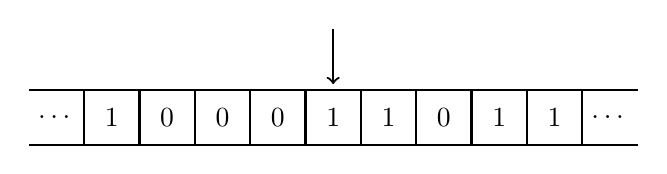
\begin{tikzpicture}
			[block/.style ={rectangle, draw=black, thick, text centered,align=center, minimum height=2em,minimum width=2.0em},
				block2/.style={
						text centered,align=center, minimum height=2em,minimum width=2.0em
					}]
			\draw[thick] (-11em,-1em) -- (-9em,-1em) -- (-9em,1em) -- (-11em,1em);
			\node[block2] at (-5*2em,0) {\ldots};

			\draw (-4*2.0em,0) node[block] {$1$};
			\draw (-3*2.0em,0) node[block] {$0$};
			\draw (-2*2.0em,0) node[block] {$0$};
			\draw (-1*2.0em,0) node[block] {$0$};
			\draw (0,0) node[block] {$1$};
			\draw (1*2.0em,0) node[block] {$1$};
			\draw (2*2.0em,0) node[block] {$0$};
			\draw (3*2.0em,0) node[block] {$1$};
			\draw (4*2.0em,0) node[block] {$1$};

			\draw[thick] (11em,-1em) -- (9em,-1em) -- (9em,1em) -- (11em,1em);
			\node[block2] at (5*2em,0) {\ldots};

			\draw[->, thick] (0,3.2em) -- (0,1.2em);
		\end{tikzpicture}
	\end{center}
	\caption{The tape and head of Turing-Post machine with oracle for $A$}
\end{figure}

\begin{definition}
	A \textit{Turing-Post program with oracle for $A$} is a sequence of Turing-Post instructions and the oracle instruction.
\end{definition}
\noindent
If $\cP$ is a Turing-Post program with oracle for $A$, then we denote by $\mathrm{lh}(\cP)$ the number of instructions in $\cP$. Moreover, if $0 \leq i < \mathrm{lh}(\cP)$, then $\cP[i]$ denotes $i$-th instruction in $\cP$.

\begin{definition}
	A \textit{state} of a Turing-Post machine with oracle for $A$ consists of:
	\begin{enumerate}[label=\textbf{(\arabic*)}, leftmargin=3.0em]
		\item the contents of all tape cells, with all but finitely many storing $0$
		\item the head position
	\end{enumerate}
	A state is \textit{initial} if $pc = 0$.
\end{definition}

\begin{definition}
	Let $\cP$ be a Turing-Post program with oracle for $A$. Suppose that a Turing-Post machine with oracle for $A$ starts in an initial state. Then \textit{execution of $\cP$ starting from this initial state} follows iterative procedure described below:
	\begin{enumerate}[label=\textbf{(\arabic*)}, leftmargin=3.0em]
		\item At the beginning of each iteration the machine reads the content of the program counter.
		\item Next the execution depends on the content of the program counter.
		      \begin{itemize}
			      \item[] If $pc < \mathrm{lh}(\cP)$, then the machine modifies contents of its cells and the program counter according to $pc$-th instruction in $\cP$.
			      \item[] If $\mathrm{lh}(\cP) \leq pc$, then the machine halts.
		      \end{itemize}
	\end{enumerate}
\end{definition}

\begin{definition}
	Let $\cP$ be a Turing-Post program with oracle for $A$. Suppose $\cP$ is executed on a Turing-Post machine with oracle for $A$ starting from some initial state. If at some point of the execution the machine halts by attempting to fetch $\mathrm{lh}(\cP)$-th instruction, then the execution of $\cP$ \textit{terminates} when started in that initial state.
\end{definition}

\begin{remark}\label{remark:relative_jumps}
	For additional flexibility we add two more Turing-Post instructions
	\begin{itemize}
		\item[] $\mathrm{JMP}+q$: increments $pc$ by $q \in \NN$
		\item[] $\mathrm{JMP}-q$: decrements $pc$ by $q \in \NN$; only valid if $q \leq pc$.
	\end{itemize}
	Note that these both instructions can be compiled into the standard $\mathrm{GO\,TO}$ instructions.
\end{remark}
\noindent
Note that Turing-Post machines and programs with oracle for $A$ are extremely simple. Actually the whole point of introducing them is to show that a computation only requires very rudimentary and finite operations.

Our goal is to show that register-machine programs with oracle for $A$ can be compiled into Turing-Post programs with oracle for $A$. To do this, we encode register states as tape states. Fix a state of register machine and assume that only the first $R \in \NN$ registers contain nonzero values. Represent this state on the tape by $R$ blocks of consecutive $1$s with each pair of consecutive blocks separated by a single $0$. The $(r+1)$-th block from the left consists of $c_r + 1$ consecutive $1$s. The head points to the first cell encoding register $0$.

\begin{figure}[H]
	\begin{center}
		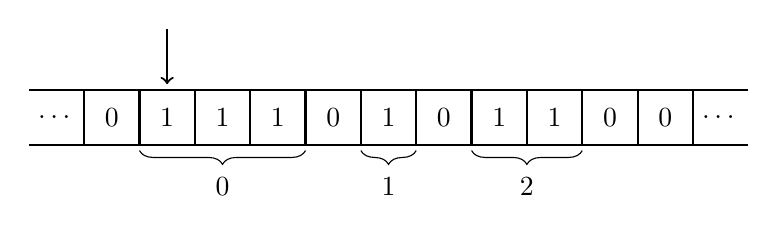
\begin{tikzpicture}
			[block/.style ={rectangle, draw=black, thick, text centered,align=center, minimum height=2em,minimum width=2.0em},
				block2/.style={
						text centered,align=center, minimum height=2em,minimum width=2.0em
					}]
			\draw[thick] (-13em,-1em) -- (-11em,-1em) -- (-11em,1em) -- (-13em,1em);
			\node[block2] at (-6*2em,0) {\ldots};

			\draw (-5*2.0em,0) node[block] {$0$};
			\draw (-4*2.0em,0) node[block] {$1$};
			\draw (-3*2.0em,0) node[block] {$1$};
			\draw (-2*2.0em,0) node[block] {$1$};
			\draw (-1*2.0em,0) node[block] {$0$};
			\draw (0,0) node[block] {$1$};
			\draw (1*2.0em,0) node[block] {$0$};
			\draw (2*2.0em,0) node[block] {$1$};
			\draw (3*2.0em,0) node[block] {$1$};
			\draw (4*2.0em,0) node[block] {$0$};
			\draw (5*2.0em,0) node[block] {$0$};

			\draw[thick] (13em,-1em) -- (11em,-1em) -- (11em,1em) -- (13em,1em);
			\node[block2] at (6*2em,0) {\ldots};

			\draw[->, thick] (-8em,3.2em) -- (-8em,1.2em);

			\draw[decorate,decoration={brace,mirror,amplitude=5pt}]
			(-4*2em-1em,-1.2em) -- (-2*2em+1em,-1.2em) node[midway,yshift=-1.5em]{};
			\draw[decorate,decoration={brace,mirror,amplitude=5pt}]
			(-1em,-1.2em) -- (1em,-1.2em) node[midway,yshift=-1.5em]{};
			\draw[decorate,decoration={brace,mirror,amplitude=5pt}]
			(2em+1em,-1.2em) -- (6em+1em,-1.2em) node[midway,yshift=-1.5em]{};


			\node[block2] at (-6em,-2.5em) {0};
			\node[block2] at (0em,-2.5em) {1};
			\node[block2] at (5em,-2.5em) {2};
		\end{tikzpicture}
	\end{center}
	\caption{The tape and head of Turing-Post machine with oracle for $A$ representing the initial state of register machine with $c_0 = 2,c_1 = 0,c_2 = 2$ and all other registers storing zeros}
\end{figure}

\begin{remark}\label{remark:different_machine_tapes_encode_the_same_register_machine_state}
	Note that under this encoding different tape states may represent the same register machine state.
\end{remark}
\noindent
Now we define some helper subroutines for Turing-Post machines with oracle for $A$.

\begin{example}\label{example:next_register}
	We define subroutine $\mathrm{NEXT\,REGISTER}$.
	\begin{itemize}
		\item[] $\mathrm{MOVE\,RIGHT}$
		\item[] $\mathrm{IS\,ZERO}$
		\item[] $\mathrm{JMP}-2$
		\item[] $\mathrm{MOVE\,RIGHT}$
	\end{itemize}
	\begin{figure}[H]
		\begin{center}
			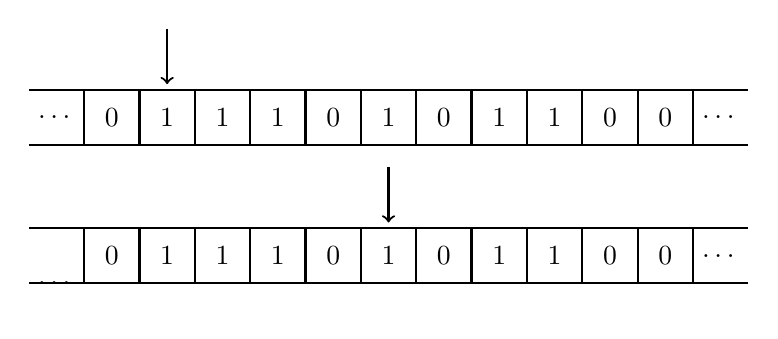
\begin{tikzpicture}
				[block/.style ={rectangle, draw=black, thick, text centered,align=center, minimum height=2em,minimum width=2.0em},
					block2/.style={
							text centered,align=center, minimum height=2em,minimum width=2.0em
						}]
				\draw[thick] (-13em,-1em) -- (-11em,-1em) -- (-11em,1em) -- (-13em,1em);
				\node[block2] at (-6*2em,0) {\ldots};

				\draw (-5*2.0em,0) node[block] {$0$};
				\draw (-4*2.0em,0) node[block] {$1$};
				\draw (-3*2.0em,0) node[block] {$1$};
				\draw (-2*2.0em,0) node[block] {$1$};
				\draw (-1*2.0em,0) node[block] {$0$};
				\draw (0,0) node[block] {$1$};
				\draw (1*2.0em,0) node[block] {$0$};
				\draw (2*2.0em,0) node[block] {$1$};
				\draw (3*2.0em,0) node[block] {$1$};
				\draw (4*2.0em,0) node[block] {$0$};
				\draw (5*2.0em,0) node[block] {$0$};

				\draw[thick] (13em,-1em) -- (11em,-1em) -- (11em,1em) -- (13em,1em);
				\node[block2] at (6*2em,0) {\ldots};

				\draw[->, thick] (-8em,3.2em) -- (-8em,1.2em);


				\draw[thick] (-13em,-6em) -- (-11em,-6em) -- (-11em,-4em) -- (-13em,-4em);
				\node[block2] at (-6*2em,-6em) {\ldots};

				\draw (-5*2.0em,-5em) node[block] {$0$};
				\draw (-4*2.0em,-5em) node[block] {$1$};
				\draw (-3*2.0em,-5em) node[block] {$1$};
				\draw (-2*2.0em,-5em) node[block] {$1$};
				\draw (-1*2.0em,-5em) node[block] {$0$};
				\draw (0,-5em) node[block] {$1$};
				\draw (1*2.0em,-5em) node[block] {$0$};
				\draw (2*2.0em,-5em) node[block] {$1$};
				\draw (3*2.0em,-5em) node[block] {$1$};
				\draw (4*2.0em,-5em) node[block] {$0$};
				\draw (5*2.0em,-5em) node[block] {$0$};

				\draw[thick] (13em,-6em) -- (11em,-6em) -- (11em,-4em) -- (13em,-4em);
				\node[block2] at (6*2em,-5em) {\ldots};

				\draw[->, thick] (0em,-1.8em) -- (0em,-3.8em);
			\end{tikzpicture}
		\end{center}
		\caption{Subroutine $\mathrm{NEXT\,REGISTER}$ moves the head to the first cell representing next register.}
	\end{figure}
\end{example}

\begin{example}\label{example:previous_register}
	We define subroutine $\mathrm{PREVIOUS\,REGISTER}$.
	\begin{itemize}
		\item[] $\mathrm{MOVE\,LEFT}$
		\item[] $\mathrm{MOVE\,LEFT}$
		\item[] $\mathrm{MOVE\,LEFT}$
		\item[] $\mathrm{IS\,ZERO}$
		\item[] $\mathrm{JMP}-2$
		\item[] $\mathrm{MOVE\,RIGHT}$
	\end{itemize}
	\begin{figure}[H]
		\begin{center}
			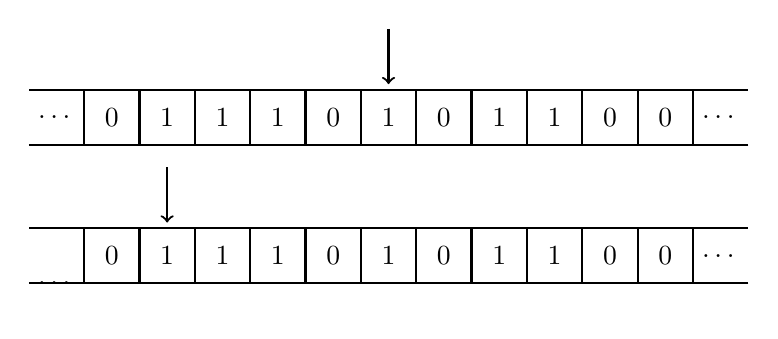
\begin{tikzpicture}
				[block/.style ={rectangle, draw=black, thick, text centered,align=center, minimum height=2em,minimum width=2.0em},
					block2/.style={
							text centered,align=center, minimum height=2em,minimum width=2.0em
						}]
				\draw[thick] (-13em,-1em) -- (-11em,-1em) -- (-11em,1em) -- (-13em,1em);
				\node[block2] at (-6*2em,0) {\ldots};

				\draw (-5*2.0em,0) node[block] {$0$};
				\draw (-4*2.0em,0) node[block] {$1$};
				\draw (-3*2.0em,0) node[block] {$1$};
				\draw (-2*2.0em,0) node[block] {$1$};
				\draw (-1*2.0em,0) node[block] {$0$};
				\draw (0,0) node[block] {$1$};
				\draw (1*2.0em,0) node[block] {$0$};
				\draw (2*2.0em,0) node[block] {$1$};
				\draw (3*2.0em,0) node[block] {$1$};
				\draw (4*2.0em,0) node[block] {$0$};
				\draw (5*2.0em,0) node[block] {$0$};

				\draw[thick] (13em,-1em) -- (11em,-1em) -- (11em,1em) -- (13em,1em);
				\node[block2] at (6*2em,0) {\ldots};

				\draw[->, thick] (0em,3.2em) -- (0em,1.2em);


				\draw[thick] (-13em,-6em) -- (-11em,-6em) -- (-11em,-4em) -- (-13em,-4em);
				\node[block2] at (-6*2em,-6em) {\ldots};

				\draw (-5*2.0em,-5em) node[block] {$0$};
				\draw (-4*2.0em,-5em) node[block] {$1$};
				\draw (-3*2.0em,-5em) node[block] {$1$};
				\draw (-2*2.0em,-5em) node[block] {$1$};
				\draw (-1*2.0em,-5em) node[block] {$0$};
				\draw (0,-5em) node[block] {$1$};
				\draw (1*2.0em,-5em) node[block] {$0$};
				\draw (2*2.0em,-5em) node[block] {$1$};
				\draw (3*2.0em,-5em) node[block] {$1$};
				\draw (4*2.0em,-5em) node[block] {$0$};
				\draw (5*2.0em,-5em) node[block] {$0$};

				\draw[thick] (13em,-6em) -- (11em,-6em) -- (11em,-4em) -- (13em,-4em);
				\node[block2] at (6*2em,-5em) {\ldots};

				\draw[->, thick] (-8em,-1.8em) -- (-8em,-3.8em);
			\end{tikzpicture}
		\end{center}\caption{Subroutine $\mathrm{PREVIOUS\,REGISTER}$ moves the head to the first cell representing the content of the previous register.}
	\end{figure}
\end{example}

\begin{example}\label{example:shift_block_of_1s_right}
	We define subroutine $\mathrm{SHIFT\,BLOCK\,OF\,1s\,RIGHT}$.
	\begin{itemize}
		\item[] $\mathrm{PRINT\,}0$
		\item[]	$\mathrm{MOVE\,RIGHT}$
		\item[]	$\mathrm{IS\,ZERO}$
		\item[]	$\mathrm{JMP}-2$
		\item[]	$\mathrm{PRINT\,}1$
		\item[] $\mathrm{MOVE\,RIGHT}$
	\end{itemize}
	\begin{figure}[H]
		\begin{center}
			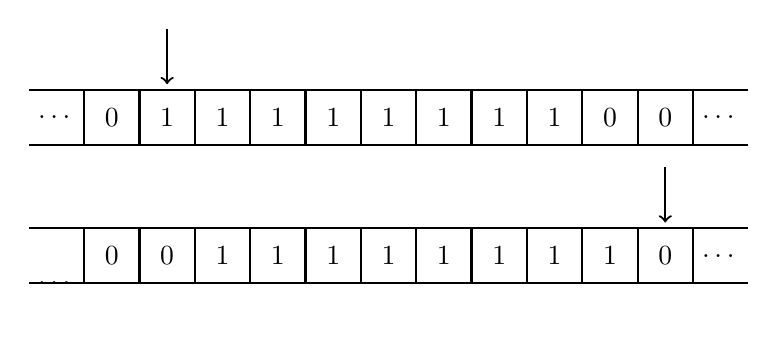
\begin{tikzpicture}
				[block/.style ={rectangle, draw=black, thick, text centered,align=center, minimum height=2em,minimum width=2.0em},
					block2/.style={
							text centered,align=center, minimum height=2em,minimum width=2.0em
						}]
				\draw[thick] (-13em,-1em) -- (-11em,-1em) -- (-11em,1em) -- (-13em,1em);
				\node[block2] at (-6*2em,0) {\ldots};

				\draw (-5*2.0em,0) node[block] {$0$};
				\draw (-4*2.0em,0) node[block] {$1$};
				\draw (-3*2.0em,0) node[block] {$1$};
				\draw (-2*2.0em,0) node[block] {$1$};
				\draw (-1*2.0em,0) node[block] {$1$};
				\draw (0,0) node[block] {$1$};
				\draw (1*2.0em,0) node[block] {$1$};
				\draw (2*2.0em,0) node[block] {$1$};
				\draw (3*2.0em,0) node[block] {$1$};
				\draw (4*2.0em,0) node[block] {$0$};
				\draw (5*2.0em,0) node[block] {$0$};

				\draw[thick] (13em,-1em) -- (11em,-1em) -- (11em,1em) -- (13em,1em);
				\node[block2] at (6*2em,0) {\ldots};

				\draw[->, thick] (-8em,3.2em) -- (-8em,1.2em);


				\draw[thick] (-13em,-6em) -- (-11em,-6em) -- (-11em,-4em) -- (-13em,-4em);
				\node[block2] at (-6*2em,-6em) {\ldots};

				\draw (-5*2.0em,-5em) node[block] {$0$};
				\draw (-4*2.0em,-5em) node[block] {$0$};
				\draw (-3*2.0em,-5em) node[block] {$1$};
				\draw (-2*2.0em,-5em) node[block] {$1$};
				\draw (-1*2.0em,-5em) node[block] {$1$};
				\draw (0,-5em) node[block] {$1$};
				\draw (1*2.0em,-5em) node[block] {$1$};
				\draw (2*2.0em,-5em) node[block] {$1$};
				\draw (3*2.0em,-5em) node[block] {$1$};
				\draw (4*2.0em,-5em) node[block] {$1$};
				\draw (5*2.0em,-5em) node[block] {$0$};

				\draw[thick] (13em,-6em) -- (11em,-6em) -- (11em,-4em) -- (13em,-4em);
				\node[block2] at (6*2em,-5em) {\ldots};

				\draw[->, thick] (10em,-1.8em) -- (10em,-3.8em);
			\end{tikzpicture}
		\end{center}
		\caption{Subroutine $\mathrm{SHIFT\,BLOCK\,OF\,1s\,RIGHT}$ shifts the block of $1$s right and moves the head to the right of the shifted block.}
	\end{figure}
\end{example}

\begin{example}\label{example:shift_block_of_1s_left}
	We define subroutine $\mathrm{SHIFT\,BLOCK\,OF\,1s\,LEFT}$.
	\begin{itemize}
		\item[] $\mathrm{MOVE\,LEFT}$
		\item[] $\mathrm{PRINT\,}1$
		\item[] $\mathrm{MOVE\,RIGHT}$
		\item[]	$\mathrm{IS\,ZERO}$
		\item[]	$\mathrm{JMP}-2$
		\item[] $\mathrm{MOVE\,LEFT}$
		\item[]	$\mathrm{PRINT\,}0$
	\end{itemize}
	\begin{figure}[H]
		\begin{center}
			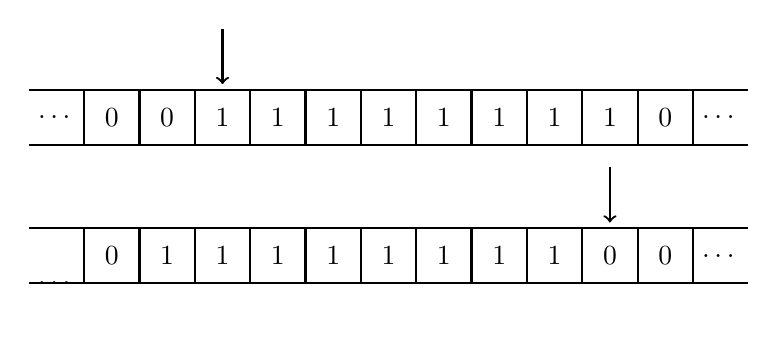
\begin{tikzpicture}
				[block/.style ={rectangle, draw=black, thick, text centered,align=center, minimum height=2em,minimum width=2.0em},
					block2/.style={
							text centered,align=center, minimum height=2em,minimum width=2.0em
						}]
				\draw[thick] (-13em,-1em) -- (-11em,-1em) -- (-11em,1em) -- (-13em,1em);
				\node[block2] at (-6*2em,0) {\ldots};

				\draw (-5*2.0em,0) node[block] {$0$};
				\draw (-4*2.0em,0) node[block] {$0$};
				\draw (-3*2.0em,0) node[block] {$1$};
				\draw (-2*2.0em,0) node[block] {$1$};
				\draw (-1*2.0em,0) node[block] {$1$};
				\draw (0,0) node[block] {$1$};
				\draw (1*2.0em,0) node[block] {$1$};
				\draw (2*2.0em,0) node[block] {$1$};
				\draw (3*2.0em,0) node[block] {$1$};
				\draw (4*2.0em,0) node[block] {$1$};
				\draw (5*2.0em,0) node[block] {$0$};

				\draw[thick] (13em,-1em) -- (11em,-1em) -- (11em,1em) -- (13em,1em);
				\node[block2] at (6*2em,0) {\ldots};

				\draw[->, thick] (-6em,3.2em) -- (-6em,1.2em);


				\draw[thick] (-13em,-6em) -- (-11em,-6em) -- (-11em,-4em) -- (-13em,-4em);
				\node[block2] at (-6*2em,-6em) {\ldots};

				\draw (-5*2.0em,-5em) node[block] {$0$};
				\draw (-4*2.0em,-5em) node[block] {$1$};
				\draw (-3*2.0em,-5em) node[block] {$1$};
				\draw (-2*2.0em,-5em) node[block] {$1$};
				\draw (-1*2.0em,-5em) node[block] {$1$};
				\draw (0,-5em) node[block] {$1$};
				\draw (1*2.0em,-5em) node[block] {$1$};
				\draw (2*2.0em,-5em) node[block] {$1$};
				\draw (3*2.0em,-5em) node[block] {$1$};
				\draw (4*2.0em,-5em) node[block] {$0$};
				\draw (5*2.0em,-5em) node[block] {$0$};

				\draw[thick] (13em,-6em) -- (11em,-6em) -- (11em,-4em) -- (13em,-4em);
				\node[block2] at (6*2em,-5em) {\ldots};

				\draw[->, thick] (8em,-1.8em) -- (8em,-3.8em);
			\end{tikzpicture}
		\end{center}
		\caption{Subroutine $\mathrm{SHIFT\,BLOCK\,OF\,1s\,LEFT}$ shifts the block of $1$s right and moves the head right to the shifted block.}
	\end{figure}
\end{example}

\begin{example}\label{example:increase_block_of_1s}
	We define subroutine $\mathrm{INCREASE\,BLOCK\,OF\,1s}$.
	\begin{itemize}
		\item[] $\mathrm{MOVE\,RIGHT}$
		\item[] $\mathrm{IS\,ZERO}$
		\item[]	$\mathrm{JMP}-2$
		\item[] $\mathrm{PRINT\,}1$
		\item[] $\mathrm{MOVE\,RIGHT}$
	\end{itemize}
	\begin{figure}[H]
		\begin{center}
			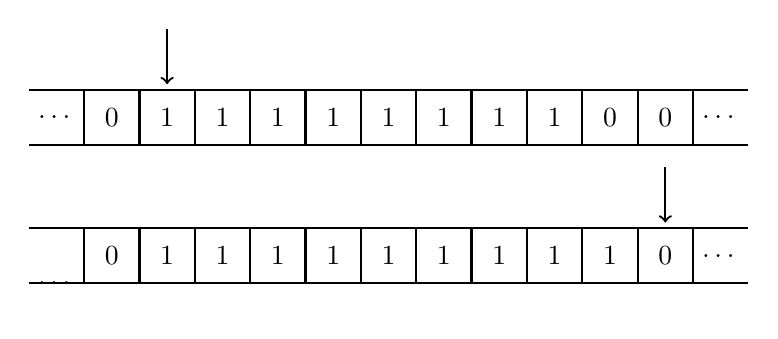
\begin{tikzpicture}
				[block/.style ={rectangle, draw=black, thick, text centered,align=center, minimum height=2em,minimum width=2.0em},
					block2/.style={
							text centered,align=center, minimum height=2em,minimum width=2.0em
						}]
				\draw[thick] (-13em,-1em) -- (-11em,-1em) -- (-11em,1em) -- (-13em,1em);
				\node[block2] at (-6*2em,0) {\ldots};

				\draw (-5*2.0em,0) node[block] {$0$};
				\draw (-4*2.0em,0) node[block] {$1$};
				\draw (-3*2.0em,0) node[block] {$1$};
				\draw (-2*2.0em,0) node[block] {$1$};
				\draw (-1*2.0em,0) node[block] {$1$};
				\draw (0,0) node[block] {$1$};
				\draw (1*2.0em,0) node[block] {$1$};
				\draw (2*2.0em,0) node[block] {$1$};
				\draw (3*2.0em,0) node[block] {$1$};
				\draw (4*2.0em,0) node[block] {$0$};
				\draw (5*2.0em,0) node[block] {$0$};

				\draw[thick] (13em,-1em) -- (11em,-1em) -- (11em,1em) -- (13em,1em);
				\node[block2] at (6*2em,0) {\ldots};

				\draw[->, thick] (-8em,3.2em) -- (-8em,1.2em);


				\draw[thick] (-13em,-6em) -- (-11em,-6em) -- (-11em,-4em) -- (-13em,-4em);
				\node[block2] at (-6*2em,-6em) {\ldots};

				\draw (-5*2.0em,-5em) node[block] {$0$};
				\draw (-4*2.0em,-5em) node[block] {$1$};
				\draw (-3*2.0em,-5em) node[block] {$1$};
				\draw (-2*2.0em,-5em) node[block] {$1$};
				\draw (-1*2.0em,-5em) node[block] {$1$};
				\draw (0,-5em) node[block] {$1$};
				\draw (1*2.0em,-5em) node[block] {$1$};
				\draw (2*2.0em,-5em) node[block] {$1$};
				\draw (3*2.0em,-5em) node[block] {$1$};
				\draw (4*2.0em,-5em) node[block] {$1$};
				\draw (5*2.0em,-5em) node[block] {$0$};

				\draw[thick] (13em,-6em) -- (11em,-6em) -- (11em,-4em) -- (13em,-4em);
				\node[block2] at (6*2em,-5em) {\ldots};

				\draw[->, thick] (10em,-1.8em) -- (10em,-3.8em);
			\end{tikzpicture}
		\end{center}
		\caption{Subroutine $\mathrm{INCREASE\,BLOCK\,OF\,1s}$ increases the block of $1$s by adding one cell on the right and moves the head to the right of the increased block.}
	\end{figure}
\end{example}

\begin{example}\label{example:decrease_block_of_1s}
	We define subroutine $\mathrm{DECREASE\,BLOCK\,OF\,1s}$.
	\begin{itemize}
		\item[] $\mathrm{MOVE\,RIGHT}$
		\item[] $\mathrm{IS\,ZERO}$
		\item[]	$\mathrm{JMP}-2$
		\item[] $\mathrm{MOVE\,LEFT}$
		\item[] $\mathrm{PRINT\,}0$
	\end{itemize}
	\begin{figure}[H]
		\begin{center}
			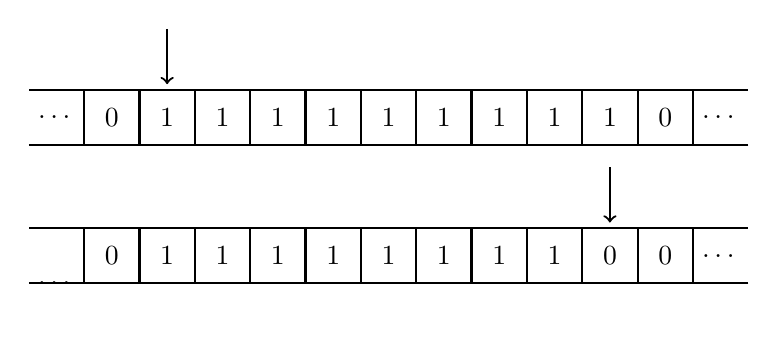
\begin{tikzpicture}
				[block/.style ={rectangle, draw=black, thick, text centered,align=center, minimum height=2em,minimum width=2.0em},
					block2/.style={
							text centered,align=center, minimum height=2em,minimum width=2.0em
						}]
				\draw[thick] (-13em,-1em) -- (-11em,-1em) -- (-11em,1em) -- (-13em,1em);
				\node[block2] at (-6*2em,0) {\ldots};

				\draw (-5*2.0em,0) node[block] {$0$};
				\draw (-4*2.0em,0) node[block] {$1$};
				\draw (-3*2.0em,0) node[block] {$1$};
				\draw (-2*2.0em,0) node[block] {$1$};
				\draw (-1*2.0em,0) node[block] {$1$};
				\draw (0,0) node[block] {$1$};
				\draw (1*2.0em,0) node[block] {$1$};
				\draw (2*2.0em,0) node[block] {$1$};
				\draw (3*2.0em,0) node[block] {$1$};
				\draw (4*2.0em,0) node[block] {$1$};
				\draw (5*2.0em,0) node[block] {$0$};

				\draw[thick] (13em,-1em) -- (11em,-1em) -- (11em,1em) -- (13em,1em);
				\node[block2] at (6*2em,0) {\ldots};

				\draw[->, thick] (-8em,3.2em) -- (-8em,1.2em);


				\draw[thick] (-13em,-6em) -- (-11em,-6em) -- (-11em,-4em) -- (-13em,-4em);
				\node[block2] at (-6*2em,-6em) {\ldots};

				\draw (-5*2.0em,-5em) node[block] {$0$};
				\draw (-4*2.0em,-5em) node[block] {$1$};
				\draw (-3*2.0em,-5em) node[block] {$1$};
				\draw (-2*2.0em,-5em) node[block] {$1$};
				\draw (-1*2.0em,-5em) node[block] {$1$};
				\draw (0,-5em) node[block] {$1$};
				\draw (1*2.0em,-5em) node[block] {$1$};
				\draw (2*2.0em,-5em) node[block] {$1$};
				\draw (3*2.0em,-5em) node[block] {$1$};
				\draw (4*2.0em,-5em) node[block] {$0$};
				\draw (5*2.0em,-5em) node[block] {$0$};

				\draw[thick] (13em,-6em) -- (11em,-6em) -- (11em,-4em) -- (13em,-4em);
				\node[block2] at (6*2em,-5em) {\ldots};

				\draw[->, thick] (8em,-1.8em) -- (8em,-3.8em);
			\end{tikzpicture}
		\end{center}\caption{Subroutine $\mathrm{DECREASE\,BLOCK\,OF\,1s}$ decreases the block of $1$s by adding one cell on the right and moves the head right to the decreased block.}
	\end{figure}
\end{example}

\begin{theorem}\label{theorem:TuringPost_simulation_of_register_machine}
	There exists a function $\Gamma$ that maps register-machine programs with oracle for $A$ to Turing-Post programs with oracle for $A$ such that the following assertions hold.
	\begin{enumerate}[label=\emph{\textbf{(\arabic*)}}, leftmargin=3.0em]
		\item Let $\cP$ be a register-machine program with oracle for $A$ and let $S$ be a state of a register machine with oracle for $A$. Suppose that executions of $\cP$ and $\Gamma(\cP)$ are started in $S$. Then the sequence of consecutive states of $\cP$ is a subsequence of the sequence of the consecutive states of $\Gamma(\cP)$.
		\item Let $\cP$ be a register-machine program with oracle for $A$ and let $S$ be a state of a register machine with oracle for $A$. Suppose that executions of $\cP$ and $\Gamma(\cP)$ are started in $S$. If the execution of $\cP$ terminates, then the execution of $\Gamma(\cP)$ terminates and they both terminate in the same state.
	\end{enumerate}
\end{theorem}
\begin{proof}
	We augment Turing-Post instructions by adding new syntactical constructs. For each number $n \in \NN$ we introduce an entity $\mathrm{SYMBOL}_n$ which represents $n$. $\mathrm{SYMBOL}_n$ for $n \in \NN$ has a twofold role.
	\begin{itemize}
		\item We replace instruction $\mathrm{GO\,TO}\,n$ by
		      $$\mathrm{GO\,TO}\,\mathrm{SYMBOL}_n$$
		      for $n\in \NN$.
		\item $\mathrm{SYMBOL}_n$ can be placed in front of instructions.
	\end{itemize}
	We now define some extra Turing-Post subroutines.

	We define subroutine $\mathrm{MOVE\,TO\,REGISTER\,}r$ for $r \in \NN$ by concatenating $r$-times the following block of instructions.
	\begin{itemize}
		\item[] $\mathrm{IS\,ZERO}$
		\item[] $\mathrm{JMP}+2$
		\item[] $\mathrm{PRINT\,}1$
		\item[] $\mathrm{NEXT\,REGISTER}$
	\end{itemize}
	and appending the block of instructions
	\begin{itemize}
		\item[] $\mathrm{IS\,ZERO}$
		\item[] $\mathrm{JMP}+2$
		\item[] $\mathrm{PRINT\,}1$
	\end{itemize}
	at the end. If the head points to the beginning of the block representing the first register, then the subroutine moves the head to the beginning of the block representing the content of register $r$. It creates any intermediate blocks if needed and the appended instructions ensure that the block representing register $r$ is properly initialized.

	We define subroutine $\mathrm{MOVE\,TO\,FIRST\,REGISTER}$ as the following sequence of instructions.
	\begin{itemize}
		\item[] $\mathrm{PREVIOUS\,REGISTER}$
		\item[] $\mathrm{IS\,ZERO}$
		\item[] $\mathrm{JMP}-1 - \mathrm{lh}\big(\mathrm{PREVIOUS\,REGISTER}\big)$
		\item[] $\mathrm{MOVE\,RIGHT}$
		\item[] $\mathrm{MOVE\,RIGHT}$
	\end{itemize}
	If the head points to the beginning of block representing some register, then the subroutine moves the head to the beginning of the block representing the first register.

	We define $I_{r,n}$ for $r,n\in \NN$ by placing $\mathrm{SYMBOL}_n$ in front of the first instruction of the following subroutine.
	\begin{enumerate}[label=\textbf{(\arabic*)}, leftmargin=3.0em]
		\item $\mathrm{MOVE\,TO\,REGISTER\,}r$
		\item $\mathrm{INCREASE\,BLOCK\,OF\,1s}$
		\item $\mathrm{IS\,ZERO}$
		\item $\mathrm{JMP}+2$
		\item $\mathrm{JMP}+2 + \mathrm{lh}\big(\mathrm{SHIFT\,BLOCK\,OF\,1s\,RIGHT}\big)$
		\item $\mathrm{SHIFT\,BLOCK\,OF\,1s\,RIGHT}$
		\item $\mathrm{JMP}-\mathrm{lh}\big(\mathrm{SHIFT\,BLOCK\,OF\,1s\,RIGHT}\big) - 3$
		\item $\mathrm{MOVE\,RIGHT}$
		\item $\mathrm{MOVE\,TO\,FIRST\,REGISTER}$
	\end{enumerate}
	We describe the effect of this subroutine on the tape of the machine. Suppose that the head points to the beginning of the block representing first register. Step \textbf{(1)} moves the head to the beginning of the block representing register $r$. Next \textbf{(2)} increases the block representing register $r$ by appending single $1$ at the end. Now \textbf{(3)}-\textbf{(7)} shift all blocks following the one representing register $r$ one cell to the right. Finally \textbf{(8)} and \textbf{(9)} return the head back to the beginning of the block representing the first register.

	We define $D_{r,n}$ for $r,n\in \NN$ by placing $\mathrm{SYMBOL}_n$ in front of the first instruction in the following subroutine.
	\begin{enumerate}[label=\textbf{(\arabic*)}, leftmargin=3.0em]
		\item $\mathrm{MOVE\,TO\,REGISTER\,}r$
		\item $\mathrm{MOVE\,RIGHT}$
		\item $\mathrm{IS\,ZERO}$
		\item $\mathrm{JMP}+3 + \mathrm{lh}\left(\mathrm{MOVE\,TO\,FIRST\,REGISTER}\right)$
		\item $\mathrm{MOVE\,RIGHT}$
		\item $\mathrm{MOVE\,TO\,FIRST\,REGISTER}$
		\item $\mathrm{GO\,TO\,}\mathrm{SYMBOL}_{n+1}$
		\item $\mathrm{DECREASE\,BLOCK\,OF\,1s}$
		\item $\mathrm{MOVE\,RIGHT}$
		\item $\mathrm{MOVE\,RIGHT}$
		\item $\mathrm{IS\,ZERO}$
		\item $\mathrm{JMP}+2$
		\item $\mathrm{JMP}+2 + \mathrm{lh}\big(\mathrm{SHIFT\,BLOCK\,OF\,1s\,LEFT}\big)$
		\item $\mathrm{SHIFT\,BLOCK\,OF\,1s\,LEFT}$
		\item $\mathrm{JMP}-\mathrm{lh}\big(\mathrm{SHIFT\,BLOCK\,OF\,1s\,LEFT}\big) - 5$
		\item $\mathrm{MOVE\,LEFT}$
		\item $\mathrm{MOVE\,TO\,FIRST\,REGISTER}$
		\item $\mathrm{GO\,TO\,}\mathrm{SYMBOL}_{n+2}$
	\end{enumerate}
	We describe the effect of this subroutine on the tape of the machine. Suppose that the head points to the beginning of the block representing first register. Step \textbf{(1)} moves the head to the beginning of the block representing register $r$. Next \textbf{(2)} and \textbf{(3)} check whether register $r$ stores zero. We have two cases.
	\begin{itemize}
		\item If register $r$ stores zero, then \textbf{(5)} and \textbf{(6)} move the head to the beginning of the block representing the first register. Next \textbf{(7)} jumps to $\mathrm{SYMBOL}_{n+1}$.
		\item If register $r$ stores a nonzero number, then \textbf{(4)} transfers the control to \textbf{(8)} which decreases the block representing register $r$ by removing rightmost $1$ and moves the head to the right of the decreased block. Next \textbf{(9)}-\textbf{(15)} shift all blocks following the block representing register $r$ one cell to the left. Steps \textbf{(16)} and \textbf{(17)} return the head to the beginning of the block representing the first register. Finally \textbf{(18)} jumps to $\mathrm{SYMBOL}_{n+2}$.
	\end{itemize}

	We define $O_{r,n}$ for $r,n\in \NN$ by placing $\mathrm{SYMBOL}_n$ in front of the first instruction in the following subroutine.
	\begin{enumerate}[label=\textbf{(\arabic*)}, leftmargin=3.0em]
		\item $\mathrm{MOVE\,TO\,REGISTER\,}r$
		\item $\mathrm{ORACLE}_A$
		\item $\mathrm{JMP\,}+\mathrm{lh}\left(\mathrm{MOVE\,TO\,FIRST\,REGISTER}\right) + 2$
		\item $\mathrm{MOVE\,TO\,FIRST\,REGISTER}$
		\item $\mathrm{GO\,TO\,}\mathrm{SYMBOL}_{n+1}$
		\item $\mathrm{MOVE\,TO\,FIRST\,REGISTER}$
		\item $\mathrm{GO\,TO\,}\mathrm{SYMBOL}_{n+2}$
	\end{enumerate}
	We describe the effect of this subroutine on the tape of the machine. Suppose that the head points to the beginning of the block representing first register. Step \textbf{(1)} moves the head to the beginning of the block representing register $r$. Next \textbf{(2)} verifies if the content of register $r$ is in $A$. We have two cases.
	\begin{itemize}
		\item If register $r$ stores an element of $A$, then \textbf{(3)} jumps to \textbf{(6)}. Next \textbf{(6)} moves the head to the beginning of the block representing the first register. Finally \textbf{(7)} jumps to $\mathrm{SYMBOL}_{n+2}$.
		\item If register $r$ does not store an element of $A$, then \textbf{(4)} moves the head to the beginning of the block representing the first register. Next \textbf{(5)} jumps to $\mathrm{SYMBOL}_{n+1}$.
	\end{itemize}

	Now we are ready to define $\Gamma$. This is done by constructing an intermediate representation.

	Suppose that $\cP$ is a register-machine program with oracle for $A$.
	\begin{itemize}
		\item If $n$-th instruction of $\cP$ is $\mathrm{INC\,}r$ for some $r\in \NN$, then we compile it to $I_{r,n}$.
		\item If $n$-th instruction of $\cP$ is $\mathrm{DEC\,}r$ for some $r\in \NN$, then we compile it to $D_{r,n}$.
		\item If $n$-th instruction of $\cP$ is $\mathrm{JUMP\,}q$ for some $q\in \ZZ$, then we compile it to $\mathrm{GO\,TO\,}\mathrm{SYMBOL}_{n+q}$.
		\item If $n$-th instruction of $\cP$ is $\mathrm{ORACLE}_A\,r$ for some $r \in \NN$, then we compile it to $\mathrm{O}_{r,n}$.
	\end{itemize}
	The concatenation of the compiled instructions in the correct order is the intermediate representation $\tilde{\cP}$ of $\cP$.

	Next for every  $\mathrm{SYMBOL}_n$ for $n\in \NN$ appearing in front of some instruction in $\tilde{\cP}$.
	\begin{enumerate}[label=\textbf{(\arabic*)}, leftmargin=3.0em]
		\item Remove it from this instruction.
		\item Replace all other occurrences of $\mathrm{SYMBOL}_n$ by the position of that instruction.
	\end{enumerate}
	Perform this procedure for all $\mathrm{SYMBOL}_n$ occurring in front of instructions of $\tilde{\cP}$. Next for every $\mathrm{SYMBOL}_{\mathrm{lh}(\cP)}$ appearing in $\tilde{\cP}$ replace it by $\mathrm{lh}(\tilde{\cP})$. If any symbols remain as parts of go-to instructions after this, then replace them by $\mathrm{lh}(\tilde{\cP}) + 1$. This transformation produces $\Gamma(\cP)$.

	According to descriptions of subroutines $I_{r,n}, D_{r,n}, O_{r,n}$ for $r,n\in \NN$ and by straightforward observation that $\mathrm{JUMP\,}q$ at $n$-th position in register-machine program is semantically equivalent to Turing-Post $\mathrm{GO\,TO\,}\mathrm{SYMBOL}_{n + q}$ for $n\in \NN$ and $q\in \ZZ$, we deduce that $\Gamma(\cP)$ satisfies the assertions in the statement of the theorem.
\end{proof}

\begin{definition}
	Let $\vec{n}\in \NN^k$ for some $k \in \NN$. Consider a state of a Turing-Post machine with oracle for $A$ consisting of $k$ contiguous blocks of $1$s separated by single $0$s such that the $i$-th block from the left contains $n_i$ ones for $1\leq i \leq k$ and the head points to the beginning of the first block. Then the machine \textit{stores} $\vec{n}$.
\end{definition}

\begin{definition}
	Let $\cP$ be a Turing-Post program with oracle for $A$ and let $f$ be a $k$-ary partial function for some $k \in \NN$. Suppose that the following assertions hold.
	\begin{enumerate}[label=\textbf{(\arabic*)}, leftmargin=3.0em]
		\item If $\vec{n}\in \NN^k$ is any $k$-tuple in the complement of the domain of $f$, then executing $\cP$ on a Turing-Post machine with oracle for $A$ initialized with $\vec{n}$ stored on the tape runs indefinitely.
		\item If $\vec{n} \in \NN^k$ is any $k$-tuple in the domain of $f$, then executing $\cP$ on a Turing-Post machine with oracle for $A$ initialized with $\vec{n}$ stored on the tape terminates and results in the state in which the tape contains single contiguous block of $f(\vec{n})$ ones and the head points to the beginning of the block.
	\end{enumerate}
	Then $f$ is \textit{Turing-Post computable relative to $A$} and $\cP$ \textit{computes} $f$.
\end{definition}

\begin{corollary}\label{corollary:register_machine_are_Turing_Post_computable}
	Each register-machine computable function relative to $A$ is Turing-Post computable relative to $A$.
\end{corollary}
\begin{proof}
	Let $f$ be a $k$-ary register-machine computable function relative to $A$ and let $\cP$ be a register-machine program with oracle for $A$ that computes $f$. Suppose that $M \in \NN$ is greater than $k$ and all registers occurring in instructions of $\cP$. Define $\mathcal{Q}$ by appending to $\cP$ instructions $\mathrm{CLEAR\,}r$ for $0 < r < M$. Then $\mathcal{Q}$ computes $f$ and clears all registers except register $0$ upon termination.

	There exists a Turing-Post program with oracle for $A$ which when initialized with $\vec{n}$ stored on the tape for $\vec{n} \in \NN^k$ terminates with the machine storing
	$$\left(1,n_1+1,...,n_k+1\right)$$
	We leave the implementation of this program as an exercise for the reader and name this subroutine $\mathrm{PREPARE\,TAPE}$.

	Next there exists a Turing-Post program with oracle for $A$ which starts with the machine storing the state of the register machine such that $c_r = 0$ for all positive $r \in \NN$ and upon termination leaves a unique block of $c_0$ ones with the head pointing to the beginning of the block. The implementation of this program is also left as an exercise. We name this subroutine $\mathrm{CLEAN\,TAPE}$.

	Finally Turing-Post program with oracle for $A$
	\begin{itemize}
		\item[] $\mathrm{PREPARE\,TAPE}$
		\item[] $\Gamma(\mathcal{Q})$
		\item[] $\mathrm{CLEAN\,TAPE}$
	\end{itemize}
	computes $f$, where $\Gamma$ is defined in Theorem \ref{theorem:TuringPost_simulation_of_register_machine}.
\end{proof}

\section{The language of arithmetic}
\noindent
In this section we fix a subset $A \subseteq \NN$.

\begin{definition}
	The \textit{language of arithmetic} is the first order language with identity whose signature consists of the following symbols:
	$$\underbrace{\bd{0}}_{\mathrm{constant}},\underbrace{<}_{\mathrm{binary\,relation\,symbol}},\underbrace{S}_{\mathrm{unary\,function\,symbol}},\underbrace{+,\cdot}_{\mathrm{binary\,function\,symbols}}$$
	We also denote this language with $\bd{Ar}$.
\end{definition}
\noindent
The intended model of $\bd{Ar}$ is $\fN = \left(\NN,0,s,<,+,\cdot\right)$ where symbols $0,<,+,\cdot$ have their usual meaning and $s$ denotes the successor function i.e. $s(n) = n + 1$ for every $n \in \NN$.

For every $n \in \NN$ the term $\underbrace{S\cdot...\cdot S}_{n\,\mathrm{times}}\bd{0}$ of $\bd{Ar}$ is denoted by $\overline{n}$.

We also fix a bijection between the first countable ordinal and the collection of variables of $\bd{Ar}$. This induces a well-ordering on variables of $\bd{Ar}$.

\begin{definition}
	The \textit{language of arithmetic relative to $A$} is the extension of $\bd{Ar}$ by $$\underbrace{r_A}_{\mathrm{unary\,relation\,symbol}}$$
	We denote this language by $\bd{Ar}_A$.
\end{definition}
\noindent
The intended model of $\bd{Ar}_A$ is the expansion of $\fN$ by interpreting $r_A$ as $A \subseteq \NN$. This model of $\bd{Ar}_A$ is denoted by $\fN_A$.

\begin{definition}
	Let $\phi$ be a formula in $\bd{Ar}_A$ and let $x_1,...,x_k$ be all free variables of $\phi$ listed according to the fixed well-order on the variables of $\bd{Ar}_A$. Then $x_1,...,x_k$ is the \textit{context} of $\phi$.
\end{definition}
\noindent
Let $\phi$ be a formula of $\bd{Ar}_A$ and let $x_1,...,x_k$ be the context of $\phi$. For $n_1,...,n_k\in \NN$ we denote by $\phi(n_1,...n_k)$ the sentence obtained from $\phi$ by substituting $x_i$ by $\overline{n}_i$ for $i=1,...,k$.

\begin{definition}
	Let $\phi$ be a formula in $\bd{Ar}_A$ and let $x_1,...,x_k$ be the context of $\phi$. Then we set
	$$\phi^{\fN_A} = \big\{(n_1,...,n_k) \in \NN^k\,\big|\,\phi(n_1,...,n_k)\mbox{ holds in }\fN\big\}$$
	Then $k$-ary relation $\phi^{\fN}\subseteq \NN^k$ is the \textit{interpretation} of $\phi$ in $\fN_A$.
\end{definition}

\begin{definition}
	Let $\phi$ and $\psi$ be formulas in $\bd{Ar}_A$. If $\phi^{\fN_A} = \psi^{\fN_A}$, then $\phi$ and $\psi$ are \textit{arithmetically equivalent}.
\end{definition}

\begin{definition}
	Let $R$ be a $k$-ary relation and let $\phi$ be a formula of $\bd{Ar}_A$. Then $R$ is \textit{definable} by $\phi$ if $\phi^{\fN_A}$ coincides with $R$.
\end{definition}

\begin{remark}\label{remark:bounded_quantifiers}
	Let $\phi$ be a formula in $\bd{Ar}_A$ and let $x,y$ be distinct variables. Then we introduce the following notation
	$$x \leq y \equiv \left(x = y\right) \vee \left(x < y\right)$$
	$$\forall_{x < y}\,\phi \equiv \forall_x\,\big(\left(y \leq x\right)\vee \phi\big),\,\exists_{x < y}\,\phi \equiv \exists_x\,\big(\left(x < y\right)\wedge \phi\big)$$
	$$\forall_{x \leq y}\,\phi \equiv \forall_x\,\big(\left(y < x\right)\vee \phi\big),\,\exists_{x \leq y}\,\phi \equiv \exists_x\,\big(\left(x \leq y\right)\wedge \phi\big)$$
\end{remark}

\section{Rudimentary and existential rudimentary formulas}
\noindent
We fix a subset $A \subseteq \NN$. In this section we introduce important class of formulas of $\bd{Ar}_A$.

\begin{definition}
	The class of \textit{rudimentary formulas relative to $A$} is the smallest class of formulas in $\bd{Ar}_A$ such that the following conditions hold.
	\begin{enumerate}[label=\textbf{(\arabic*)}, leftmargin=3.0em]
		\item Every atomic formula is rudimentary relative to $A$.
		\item If $\phi,\psi$ are rudimentary formulas relative to $A$, then
		      $$\left(\phi \wedge \psi\right),\left(\phi \vee \psi\right)$$
		      are rudimentary relative to $A$.
		\item If $\phi$ is a rudimentary formula relative to $A$, then $\left(\neg \phi\right)$ is rudimentary relative to $A$.
		\item if $\phi$ is a rudimentary formula relative to $A$ and $x,y$ are variables, then also
		      $$\forall_{x < y}\,\phi,\,\forall_{x \leq y}\,\phi,\,\exists_{x < y}\,\phi,\,\exists_{x \leq y}\,\phi$$
		      are rudimentary relative to $A$.
	\end{enumerate}
\end{definition}

\begin{definition}
	Let $\phi$ be a rudimentary formula relative to $A$ and let $x$ be a variable. Then $\exists_x\,\phi$ is a \textit{$\exists$-rudimentary formula relative to $A$}.
\end{definition}

\begin{proposition}\label{proposition:extensional_properties_of_existential_rudimentary_formulas}
	The following assertions hold.
	\begin{enumerate}[label=\emph{\textbf{(\arabic*)}}, leftmargin=3.0em]
		\item If $\phi$ is $\exists$-rudimentary formula relative to $A$ and $x$ is variable, then $\exists_x\,\phi$ is arithmetically equivalent to $\exists$-rudimentary formula relative to $A$.
		\item If $\phi$ and $\psi$ are $\exists$-rudimentary formulas relative to $A$, then formulas $\left(\phi \wedge \psi\right)$ and $\left(\phi \vee \psi\right)$ are arithmetically equivalent to $\exists$-rudimentary formulas relative to $A$.
		\item If $\phi$ is $\exists$-rudimentary formula relative to $A$ and $x,y$ are variables, then formulas
		      $$\forall_{x < y}\,\phi,\,\forall_{x \leq y}\,\phi,\,\exists_{x < y}\,\phi,\,\exists_{x \leq y}\,\phi$$
		      are arithmetically equivalent to $\exists$-rudimentary formulas relative to $A$.
	\end{enumerate}
\end{proposition}
\begin{proof}
	Assume that $\phi$ is $\exists$-rudimentary relative to $A$. Then $\phi \equiv \exists_z\,\theta$ for some rudimentary formula $\theta$ relative to $A$ and variable $z$. Pick variable $t$ different from both $x, z$ and all variables occurring in $\theta$. Then $\exists_x\exists_z\,\theta$ is arithmetically equivalent to $\exists$-rudimentary formula $\exists_t\exists_{x < t}\exists_{z < t}\,\theta$ relative to $A$. This proves \textbf{(1)}.

	Now suppose that $\phi$ and $\psi$ are $\exists$-rudimentary relative to $A$. Then there exist rudimentary formulas $\theta, \eta$ relative to $A$ and variables $x, y$ such that $\phi \equiv \exists_x\,\theta,\,\psi \equiv \exists_y\,\eta$.
	Now pick variable $t$ different from $x,y$ and all variables occurring in $\theta$ and $\eta$. Then
	$$\left(\phi \wedge \psi\right) \equiv \left(\exists_x\,\theta \wedge \exists_y\,\eta\right)$$
	is arithmetically equivalent to $\exists$-rudimentary formula
	$$\exists_t\big(\exists_{x < t}\,\theta \wedge \exists_{y < t}\,\eta\big)$$
	relative to $A$. Similar argument works for $\vee$. This proves \textbf{(2)}.

	Assume that $\phi$ is $\exists$-rudimentary relative to $A$. Then $\phi \equiv \exists_z\,\theta$ for some rudimentary formula $\theta$ and variable $z$. Pick variable $t$ different from $z, x, y$ and all variables occurring with $\theta$. Then
	$$\forall_{x < y}\exists_z\,\theta$$
	is arithmetically equivalent to $\exists$-rudimentary formula
	$$\exists_t\forall_{x < y}\exists_{z < t}\,\theta$$
  relative to $A$. Similar argument works with $\forall_{x \leq y}\,\phi$. Consider now $\exists_{x < y}\,\phi$. By definition this formula is
	$$\exists_x\,\big(\left(x < y\right)\wedge \phi\big)$$
  and hence it is arithmetically equivalent to $\exists$-rudimentary relative to $A$ by \textbf{(1)} and \textbf{(2)}. Similar argument works with $\exists_{x \leq y}\,\phi$. This completes the proof of \textbf{(3)}.
\end{proof}

\section{Existential rudimentary functions and relations}
\noindent
We fix a subset $A \subseteq \NN$.

\begin{definition}
	Let $R$ be a $k$-ary relation definable by $\exists$-rudimentary formula relative to $A$. Then $R$ is an $\exists$-\textit{rudimentary relative to $A$}.
\end{definition}

\begin{definition}
	Let $f$ be a $k$-ary partial function such that $\Gamma_f$ is $\exists$-rudimentary relation relative to $A$. Then $f$ is an $\exists$-\textit{rudimentary relative to $A$}.
\end{definition}

\begin{remark}\label{remark:}
	Rudimentary and $\exists$-rudimentary formulas relative to $\emptyset$ are referred to simply as rudimentary and $\exists$-rudimentary. Similarly $\exists$-rudimentary relations and functions relative to $\emptyset$ are referred to as $\exists$-rudimentary relations and functions.
\end{remark}

\begin{fact}\label{fact:basic_primitive_recursive_functions_are_existential_rudimentary}
	The following functions are $\exists$-rudimentary.
	\begin{enumerate}[label=\emph{\textbf{(\arabic*)}}, leftmargin=3.0em]
		\item The zero $k$-ary function for every $k \in \NN$.
		\item $I^i_k$ for every $k \in \NN$ and every $1 \leq i \leq k$.
		\item The successor, the addition and the multiplication.
	\end{enumerate}
\end{fact}
\begin{proof}
	The proof is left for the reader.
\end{proof}

\begin{fact}\label{fact:characteristic_function_of_oracle_set_is_existential_rudimentary_relatively}
	The function $\mathbb{1}_A$ is $\exists$-rudimentary relative to $A$.
\end{fact}
\begin{proof}
	Indeed, the formula
	$$\left(y = \overline{1} \wedge r_Ax\right)\vee \left(y = \bd{0} \wedge \left(\neg r_Ax\right)\right)$$
	is $\exists$-rudimentary relative to $A$ and defines $\mathbb{1}_A$.
\end{proof}

\begin{proposition}\label{proposition:class_of_existential_rudimentary_functions_is_closed_under_composition}
	The class of $\exists$-rudimentary functions relative to $A$ is closed under composition.
\end{proposition}
\begin{proof}
	Suppose that $f_1,...,f_k$ are $l$-ary $\exists$-rudimentary functions relative to $A$ and $g$ is a $k$-ary $\exists$-rudimentary function relative to $A$. Let $\phi_{1},...,\phi_{k}$ be $\exists$-rudimentary formulas relative to $A$ defining $f_1,...,f_k$. By renaming free variables we may assume that the context of $\phi_{i}$ is $x_1,...,x_l,y_i$ for $i = 1,...,k$. Then
	$$f_i(m_1,...,m_l) = m\,\Leftrightarrow\,\phi_{i}\left(m_1,...,m_l,m\right)\mbox{ holds in }\fN$$
	for every $m_1,...,m_l,m\in \NN$ and $i = 1,...,k$. Let $\phi$ be an $\exists$-rudimentary formula relative to $A$ defining $g$. By renaming free variables we may assume that the context of $\phi$ is $y_1,...,y_k,y$ and
	$$g(n_1,...,n_k) = n\,\Leftrightarrow\,\phi\left(n_1,...,n_k,n\right)\mbox{ holds in }\fN$$
	for all $n_1,...,n_k,n\in \NN$. Then
	$$\exists_{y_1}\exists_{y_2}...\exists_{y_k}\,\left(\phi_{1}\wedge ... \wedge \phi_{k}\wedge \phi\right)$$
	is a formula of $\bd{Ar}_A$ which defines the composition of $g$ with $f_1,...,f_k$. By Proposition \ref{proposition:extensional_properties_of_existential_rudimentary_formulas} we infer that the formula above is arithmetically equivalent to $\exists$-rudimentary formula relative to $A$. Thus the composition of $g$ with $f_1,...,f_k$ is $\exists$-rudimentary relative to $A$. This completes the proof.
\end{proof}
\noindent
Now we prove nontrivial result proved in \cite{godel1931formal}.

\begin{theorem}[G{\"o}del]\label{theorem:existential_rudimentary_are_closed_under_primitive_recursion}
	The class of $\exists$-rudimentary functions relative to $A$ is closed under primitive recursion.
\end{theorem}
\noindent
We first need to prove the following interesting result.

\begin{lemma}[Beta function]\label{lemma:Godels_beta_lemma}
	There exists $\exists$-rudimentary total $3$-ary function $\beta$ such that for every $n \in \NN$ and every sequence $a_0,...,a_n \in \NN$ there exist $a, b \in \NN$ such that
	$$\beta(a,b,i) = a_i$$
	for $0 \leq i \leq n$.
\end{lemma}
\begin{proof}[Proof of the lemma]
	Consider a rudimentary formula
	$$\exists_t\bigg(\forall_{z \leq t}\big(z\cdot y < x\big)\wedge \left(x \leq S(t)\cdot y\right) \wedge \left(r + t\cdot y = x\right)\bigg)$$
	in the context $x, y, r$. Then this formula defines a $2$-ary function which maps a pair $(n, m)$ to the remainder of division of $n$ by $m$.

	Now we define
	$$\beta\left(n_1,n_2,n_3\right) = \mathrm{rem}\big(n_1,\left(n_3 + 1\right)\cdot n_2 + 1\big)$$
	Then $\beta$ is $3$-ary $\exists$-rudimentary function by Fact \ref{fact:basic_primitive_recursive_functions_are_existential_rudimentary} and Proposition \ref{proposition:class_of_existential_rudimentary_functions_is_closed_under_composition}.

	Now pick $n \in \NN$ and a sequence $a_0,...,a_n \in \NN$. Suppose that
	$$\max\left(a_0,...,a_n, n\right) \leq m$$
	for some $m \in \NN$. Then numbers
	$$\left(i + 1\right)\cdot m! + 1$$
	for $0 \leq i \leq n$ are pairwise coprime. According to Chinese remainder theorem there exists $a \in \NN$ such that
	$$\beta(a, m!, i) = \mathrm{rem}\big(a, \left(i + 1\right)\cdot m! + 1\big) = a_i$$
	for $0\leq i \leq n$. This completes the proof.
\end{proof}

\begin{proof}[Proof of the theorem]
	Suppose that $g$ is $(k+2)$-ary $\exists$-rudimentary function relative to $A$ and $f$ is $k$-ary $\exists$-rudimentary function relative to $A$. Let $\phi$ be an $\exists$-rudimentary formula that defines $\beta$ from Lemma \ref{lemma:Godels_beta_lemma}. Without loss of generality assume that the context of $\phi$ is $z_1,z_2,z_3,z$ and
	$$\beta(n_1,n_2,n_3) = n\,\Leftrightarrow\,\phi(n_1,n_2,n_3,n)\mbox{ holds in }\fN$$
	for all $n_1,n_2,n_3,n\in \NN$. Let $\theta$ be an $\exists$-rudimentary formula relative to $A$ with context $x_1,...,x_k,y,z,w$ such that
	$$g(n_1,...,n_k,m,n) = l\,\Leftrightarrow\,\theta(n_1,...,n_k,m,n,l)\mbox{ holds in }\fN$$
	for all $n_1,...,n_k,m,n,l\in \NN$. Let $\psi$ be an $\exists$-rudimentary formula relative to $A$ with context $x_1,...,x_k,u$ such that
	$$f(n_1,...,n_k) = l\,\Leftrightarrow\,\psi(n_1,...,n_k,l)\mbox{ holds in }\fN$$
	for all $n_1,...,n_k,l\in \NN$. Moreover, without loss of generality we may assume that all variables
	$$z_1,z_2,z_3,x_1,...,x_k,y,z,w,u$$
	are distinct. Let $t$ be a variable distinct from all these variables. Consider the formula
	$$\exists_{z_1}\exists_{z_2}\bigg(\exists_u\big([\phi]^{z_3,z}_{\bd{0},u}\wedge \psi\big)\wedge \forall_{t < y}\exists_w\exists_z\big([\phi]^{z_3}_{t}\wedge [\theta]^y_t \wedge [\phi]^{z_3,z}_{S(t),w}\big)\wedge [\phi]^{z_3}_y\bigg)$$
	Proposition \ref{proposition:extensional_properties_of_existential_rudimentary_formulas} shows that the formula above is arithmetically equivalent to an $\exists$-rudimentary formula relative to $A$. By Lemma \ref{lemma:Godels_beta_lemma} we infer that the formula defines $(k+1)$-ary function obtained by primitive recursion from $g$ and $f$.
\end{proof}

\begin{corollary}\label{corollary:primitive_recursive_functions_and_relations_are_existential_rudimentary}
	The following assertions hold.
	\begin{enumerate}[label=\emph{\textbf{(\arabic*)}}, leftmargin=3.0em]
		\item Each primitive recursive function relative to $A$ is $\exists$-rudimentary relative to $A$.
		\item Each primitive recursive relation relative to $A$ is $\exists$-rudimentary relative to $A$.
	\end{enumerate}
\end{corollary}
\begin{proof}
	The assertion \textbf{(1)} follows immediately from Fact \ref{fact:basic_primitive_recursive_functions_are_existential_rudimentary}, Fact \ref{fact:characteristic_function_of_oracle_set_is_existential_rudimentary_relatively}, Proposition \ref{proposition:class_of_existential_rudimentary_functions_is_closed_under_composition} and Theorem \ref{theorem:existential_rudimentary_are_closed_under_primitive_recursion}.

	Let $R$ be a $k$-ary primitive recursive relation relative to $A$ for some $k \in \NN$. Then there exists an $\exists$-rudimentary formula $\phi$ relative to $A$ with context $x_1,...,x_{k},y$ that defines $\mathbb{1}_R$. Thus $[\phi]^{y}_{\overline{1}}$ defines $R$. Hence $R$ is $\exists$-rudimentary relative to $A$. This completes the proof of \textbf{(2)}.
\end{proof}

\section{Turing-Post programs and existential rudimentary formulas}
\noindent
We fix a subset $A \subseteq \NN$.

\begin{definition}
	Let $S$ be a state of a Turing-Post machine with oracle for $A$. Let $(l,r)$ be a pair of numbers such that the following assertions hold.
	\begin{enumerate}[label=\textbf{(\arabic*)}, leftmargin=3.0em]
		\item The string of symbols in the cells to the left of the head forms the binary expansion of $l$.
		\item The string of symbols in the cells to the right of the head, including the cell under the head and with the largest infinite block of trailing zeros removed, forms the reversed binary expansion of $r$.
	\end{enumerate}
	Then the number $\pmb{[}l,r\pmb{]}$ is \textit{Wang encoding} of $S$. We denote it by $W(S)$.
\end{definition}

\begin{theorem}\label{theorem:existential_rudimentary_formula_which_describes_execution_of_Turing_Post_program}
	There exists a function $\Gamma$ that maps Turing-Post programs with oracle for $A$ to $\exists$-rudimentary formulas relative to $A$ such that the following assertions hold.
	\begin{enumerate}[label=\emph{\textbf{(\arabic*)}}, leftmargin=3.0em]
		\item Let $\cP$ be a Turing-Post program with oracle for $A$. Then $\Gamma(\cP)$ is a formula with context $x_t,x_m,y_{pc},y_m$.
		\item For all $t,i_m,o_{pc},o_m \in \NN$ the sentence
		      $$\Gamma(\cP)(t,i_m,o_{pc},o_m)$$
		      holds in $\fN$ if and only if the execution of $\cP$ on the Turing-Post machine with oracle for $A$ started from the state with Wang encoding $i_m$ does not halt before step $t$ and after this step the state of the machine is encoded by $o_m$ and the program counter stores $o_{pc}$.
	\end{enumerate}
\end{theorem}
\noindent
For the proof we need the following result.

\begin{lemma}
	For each $n \in \NN$ let $\mathrm{t}(n)$ be a number such that the binary expansion of $n$ starts with
	$$\underbrace{1...1}_{\mathrm{t}(n)}0$$
	Then $\mathrm{t}$ is primitive recursive function.
\end{lemma}
\begin{proof}[Proof of the lemma]
	Consider binary relation
	$$\mathrm{trailingOnes} = \bigg\{(n,l)\in \NN^2\,\bigg|\,2^{l+1}\mid n\dotminus \left(2^{l+1} - 1\right)\bigg\}$$
	Note that $(n,l) \in \mathrm{trailingOnes}$ if and only if the binary expansion of $n$ starts with $\underbrace{1...1}_{l}$. Observe that
	$$\mathrm{t}(n) = \mu_{l\leq n}\bigg[(n,l) \not \in \mathrm{trailingOnes}\bigg]$$
	for every $n \in \NN$. This completes the proof.
\end{proof}

\begin{proof}[Proof of the theorem]
	We need some helper functions that describe operations of the Turing-Post machine with oracle for $A$ executing $\cP$.

	We define a function $\mathrm{oracle}_A$ by formula
	$$\mathrm{oracle}_A(i_{pc},i_m) = \begin{cases}
			i_{pc} + 1 & \mbox{ if }\mathrm{t}\left(i_m[1]\right) = 0                                                                               \\
			i_{pc} + 1 & \mbox{ if }\mathrm{t}\left(i_m[1]\right) > 0\mbox{ and }\mathbb{1}_A\big(\mathrm{t}\left(i_m[1]\right)\dotminus 1\big) = 0 \\
			i_{pc} + 2 & \mbox{ otherwise }                                                                                                         \\
		\end{cases}$$
	for every $i_{pc},i_m \in \NN$. Suppose that $i_m$ is the Wang encoding of a state and $i_{pc}$ is the content of the program counter of the machine. Then $\mathrm{oracleStep}_A(i_{pc},i_m)$ is the content of the program counter after the execution of the oracle instruction for $A$.

	We define a function $\mathrm{nextProgCounter}_{\cP}$ by formula
	$$\mathrm{nextProgCounter}_{\cP}(i_{pc}, i_{m}) = \begin{cases}
			i_{pc} + 1                    & \mbox{ if }i_{pc} < \mathrm{lh}(\cP)\mbox{ and }\cP[i_{pc}] = \mathrm{PRINT\,}0,\mathrm{PRINT\,}1         \\
			i_{pc} + 1                    & \mbox{ if }i_{pc} < \mathrm{lh}(\cP)\mbox{ and }\cP[i_{pc}] = \mathrm{MOVE\,LEFT}                         \\
			i_{pc} + 1                    & \mbox{ if }i_{pc} < \mathrm{lh}(\cP)\mbox{ and }\cP[i_{pc}] = \mathrm{MOVE\,RIGHT}                        \\

			i_{pc} + 1                    & \mbox{ if }i_{pc} < \mathrm{lh}(\cP)\mbox{ and }\cP[i_{pc}] = \mathrm{IS\,ZERO}\mbox{ and }2\mid i_{m}[1] \\
			i_{pc} + 2                    & \mbox{ if }i_{pc} < \mathrm{lh}(\cP)\mbox{ and }\cP[i_{pc}] = \mathrm{IS\,ZERO}\mbox{ and }2 \nmid i_m[1] \\
			n                             & \mbox{ if }i_{pc} < \mathrm{lh}(\cP)\mbox{ and }\cP[i_{pc}] = \mathrm{GO\,TO\,}n\mbox{ for }n\in \NN      \\
			\mathrm{oracle}_A(i_{pc},i_m) & \mbox{ if }i_{pc} < \mathrm{lh}(\cP)\mbox{ and }\cP[i_{pc}] = \mathrm{ORACLE}_A                           \\
			\mathrm{lh}(\cP) + 1          & \mbox{ otherwise }                                                                                        \\
		\end{cases}$$
	for every $i_{pc},i_m\in \NN$. Suppose that $i_m$ is the Wang encoding of a state and $i_{pc}$ is the content of the program counter of the machine. We have two cases.
	\begin{itemize}
		\item If $i_{pc} < \mathrm{lh}(\cP)$, then $\mathrm{nextProgCounter}_{\cP}(i_m,i_{pc})$ returns the content of the program counter after executing $\cP[i_{pc}]$ on the machine in the state described by $i_{m}$.
		\item If $\mathrm{lh}(\cP) \leq i_{pc}$, then $\mathrm{nextProgCounter}_{\cP}(i_m,i_{pc}) = \mathrm{lh}(\cP) + 1$.
	\end{itemize}

	We define a function $\mathrm{nextState}_{\cP}$ by formula
	$$\mathrm{nextState}_{\cP}(i_{pc}, i_{m}) = \begin{cases}
			\pmb{[}i_m[0],i_m[1] \dotminus 1\pmb{]} & \mbox{ if }i_{pc} < \mathrm{lh}(\cP)\mbox{ and }\cP[i_{pc}] = \mathrm{PRINT\,}0\mbox{ and }2 \nmid i_m[1] \\
			\pmb{[}i_m[0],i_m[1] + 1\pmb{]}         & \mbox{ if }i_{pc} < \mathrm{lh}(\cP)\mbox{ and }\cP[i_{pc}] = \mathrm{PRINT\,}1\mbox{ and }2 \mid i_m[1]  \\
			i_m                                     & \mbox{ otherwise }                                                                                        \\
		\end{cases}$$
	for every $i_{pc},i_m \in \NN$. Suppose that $i_m$ is the Wang encoding of a state and $i_{pc}$ is the content of the program counter the machine pointing to an instruction in $\cP$. Then $\mathrm{nextState}_{\cP}(i_m,i_{pc})$ returns the Wang encoding of the machine state after executing $\cP[i_{pc}]$ on the machine in the state described by $i_{m}$.

	We define function $\mathrm{next}_{\cP}$ by formula
	$$\mathrm{next}_{\cP}(j, s) = \pmb{[}\mathrm{nextProgCounter}_{\cP}(s[0], s[1]),\mathrm{nextState}_{\cP}(s[0], s[1])\pmb{]}$$
	for every $j,s\in \NN$.

	Finally, the function $\mathrm{snapshot}_{\cP}$ is obtained by primitive recursion from $\mathrm{next}_{\cP}$ and the function given by formula $i_m \mapsto \pmb{[}0,i_m\pmb{]}$ for every $i_m \in \NN$. Suppose that $i_m$ is the Wang encoding of a state of the machine and $t \in \NN$. Assume that the execution of $\cP$ starts in a state encoded by $i_m$ with the program counter pointing to the first instruction of $\cP$. If the execution does not halt before step $t$, then
	$$\mathrm{snapshot}_{\cP}(t,i_m)[0],\,\mathrm{snapshot}_{\cP}(t,i_m)[1]$$
	are, respectively, the content of program counter and the Wang encoding of the state of the machine after $t$-th step of the execution. If the execution halts before step $t$, then
	$$\mathrm{snapshot}_{\cP}(t,i_m)[0] = \mathrm{lh}(\cP) + 1$$
	These facts follow from descriptions of $\mathrm{nextProgCounter}_{\cP}$ and $\mathrm{nextState}_{\cP}$.

	Now we prove the theorem. Note that $\mathrm{oracle}_A$ is primitive recursive relative to $A$. Hence $\mathrm{nextProgCounter}_{\cP}$ is primitive recursive relative to $A$ and $\mathrm{nextState}_{\cP}$ is primitive recursive. Thus $\mathrm{snapshot}_{\cP}$ is primitive recursive relative to $A$. Next we define a relation
	$$\big\{(t,i_m,o_{pc},o_m)\,\big|\,\mathrm{snapshot}_{\cP}(t,i_m)[0] = o_{pc} \leq \mathrm{lh}(\cP)\mbox{ and }\mathrm{snapshot}_{\cP}(t,i_m)[1] = o_m\big\}$$
	This relation is primitive recursive relative to $A$. By Corollary \ref{corollary:primitive_recursive_functions_and_relations_are_existential_rudimentary} there exists an $\exists$-rudimentary formula $\Gamma(\cP)$ relative to $A$ with context $x_t,x_m,y_{pc},y_m$ that defines the relation above. According to description of $\mathrm{snapshot}_{\cP}$ the formula $\Gamma(\cP)$ satisfies the statement.
\end{proof}

\begin{theorem}\label{theorem:each_Turing_Post_computable_function_is_existential_rudimentary}
	Each Turing-Post computable function relative to $A$ is $\exists$-rudimentary relative to $A$.
\end{theorem}
\noindent
For the proof we need the following results.

\begin{lemma}\label{lemma:Wang_encoding_is_primitive_recursive}
	For each $k \in \NN$ there exists a primitive recursive function that maps $\vec{n} \in \NN^k$ into the Wang encoding of the tape of a Turing-Post machine storing $\vec{n}$.
\end{lemma}
\begin{proof}[Proof of the lemma]
	Left for the reader as an exercise.
\end{proof}

\begin{lemma}\label{lemma:inverse_Wang_encoding_of_single_unary_number_is_primitive_recursive}
	Let $U_l$ be the state of the Turing-Post machine in which the tape stores a single block of $l$ consecutive $1$s and the head is pointing to the beginning of the block for some $l \in \NN$. Then the function
	$$n \mapsto \begin{cases}
			l & \mbox{ if }n = W\left(U_l\right)\mbox{ for some }l\in \NN \\
			0 & \mbox{ otherwise }
		\end{cases}
	$$
	is primitive recursive.
\end{lemma}
\begin{proof}[Proof of the lemma]
	We have
	$$W(U_l) = \pmb{[}0, 2^{l+1} - 1\pmb{]}$$
	for every $l \in \NN$. Thus $n = W(U_l)$ for some $l \in \NN$ if and only if $l = e_2(n[1] + 1) \dotminus 1$ and $n = \pmb{[}0,2^{l+1} - 1\pmb{]}$. This implies that the function in the statement is given by
	$$n \mapsto \begin{cases}
			e_2(n[1] + 1) \dotminus 1 & \mbox{ if }n = \pmb{[}0,2^{e_2(n[1] + 1) \dotminus 1} \dotminus 1\pmb{]} \\
			0                         & \mbox{ otherwise }                                                       \\
		\end{cases}$$
	and hence is primitive recursive.
\end{proof}

\begin{proof}[Proof of the theorem]
	Let $f$ be a $k$-ary Turing-Post computable function relative to $A$ for some $k \in \NN$ and let $\cP$ be a Turing-Post program with oracle for $A$ that computes $f$. For shorthand we denote $\mathrm{lh}(\cP)$ by $l_{\cP}$. By Lemma \ref{lemma:Wang_encoding_is_primitive_recursive} and Corollary \ref{corollary:primitive_recursive_functions_and_relations_are_existential_rudimentary} there exists an $\exists$-rudimentary formula $\eta$ with context $x_1,...x_k,z$ such that for every $\vec{n} \in \NN^k$ the sentence
	$$\eta(n_1,...,n_k,i_m)$$
	holds in $\fN$ if and only if $i_m$ is the Wang encoding of the Turing-Post machine with oracle for $A$ that stores $\vec{n}$. Similarly by Lemma \ref{lemma:inverse_Wang_encoding_of_single_unary_number_is_primitive_recursive} and Corollary \ref{corollary:primitive_recursive_functions_and_relations_are_existential_rudimentary} there exists $\exists$-rudimentary formula $\zeta$ with context $y_m,y$ such that for every $(n,l) \in \NN$ the sentence
	$$\zeta(n,l)$$
	holds in $\fN$ if and only if $n = U_l$.

	Without loss of generality we may assume that variables
	$$x_1,...,x_k,z,x_t,x_m,y_{pc},y_m,y$$
	are distinct and correctly ordered according to the well-order on $\bd{Ar}_A$. Next we consider the formula
	$$\phi_f \equiv \exists_{x_m}\exists_{x_t}\exists_{y_m}\big([\eta]^z_{x_m} \wedge [\Gamma(\cP)]^{y_{pc}}_{\overline{l_{\cP}}}\wedge \zeta\big)$$
	Theorem \ref{theorem:existential_rudimentary_formula_which_describes_execution_of_Turing_Post_program} implies that $\phi_f$ is an $\exists$-rudimentary formula relative to $A$ with context $x_1,...,x_k,y$ such that for every $\vec{n} \in \NN^k$ and $l\in \NN$ the sentence
	$$\phi_f(n_1,...,n_k,l)$$
	holds in $\fN$ if and only if $f(\vec{n}) = l$.	This proves that $f$ is $\exists$-rudimentary relative to $A$.
\end{proof}


















































































\small
\bibliographystyle{apalike}
\bibliography{../zzz}



\end{document}
